% Options for packages loaded elsewhere
\PassOptionsToPackage{unicode}{hyperref}
\PassOptionsToPackage{hyphens}{url}
\PassOptionsToPackage{dvipsnames,svgnames,x11names}{xcolor}
%
\documentclass[
  letterpaper,
  DIV=11,
  numbers=noendperiod]{scrartcl}

\usepackage{amsmath,amssymb}
\usepackage{iftex}
\ifPDFTeX
  \usepackage[T1]{fontenc}
  \usepackage[utf8]{inputenc}
  \usepackage{textcomp} % provide euro and other symbols
\else % if luatex or xetex
  \usepackage{unicode-math}
  \defaultfontfeatures{Scale=MatchLowercase}
  \defaultfontfeatures[\rmfamily]{Ligatures=TeX,Scale=1}
\fi
\usepackage{lmodern}
\ifPDFTeX\else  
    % xetex/luatex font selection
\fi
% Use upquote if available, for straight quotes in verbatim environments
\IfFileExists{upquote.sty}{\usepackage{upquote}}{}
\IfFileExists{microtype.sty}{% use microtype if available
  \usepackage[]{microtype}
  \UseMicrotypeSet[protrusion]{basicmath} % disable protrusion for tt fonts
}{}
\makeatletter
\@ifundefined{KOMAClassName}{% if non-KOMA class
  \IfFileExists{parskip.sty}{%
    \usepackage{parskip}
  }{% else
    \setlength{\parindent}{0pt}
    \setlength{\parskip}{6pt plus 2pt minus 1pt}}
}{% if KOMA class
  \KOMAoptions{parskip=half}}
\makeatother
\usepackage{xcolor}
\setlength{\emergencystretch}{3em} % prevent overfull lines
\setcounter{secnumdepth}{-\maxdimen} % remove section numbering
% Make \paragraph and \subparagraph free-standing
\ifx\paragraph\undefined\else
  \let\oldparagraph\paragraph
  \renewcommand{\paragraph}[1]{\oldparagraph{#1}\mbox{}}
\fi
\ifx\subparagraph\undefined\else
  \let\oldsubparagraph\subparagraph
  \renewcommand{\subparagraph}[1]{\oldsubparagraph{#1}\mbox{}}
\fi


\providecommand{\tightlist}{%
  \setlength{\itemsep}{0pt}\setlength{\parskip}{0pt}}\usepackage{longtable,booktabs,array}
\usepackage{calc} % for calculating minipage widths
% Correct order of tables after \paragraph or \subparagraph
\usepackage{etoolbox}
\makeatletter
\patchcmd\longtable{\par}{\if@noskipsec\mbox{}\fi\par}{}{}
\makeatother
% Allow footnotes in longtable head/foot
\IfFileExists{footnotehyper.sty}{\usepackage{footnotehyper}}{\usepackage{footnote}}
\makesavenoteenv{longtable}
\usepackage{graphicx}
\makeatletter
\def\maxwidth{\ifdim\Gin@nat@width>\linewidth\linewidth\else\Gin@nat@width\fi}
\def\maxheight{\ifdim\Gin@nat@height>\textheight\textheight\else\Gin@nat@height\fi}
\makeatother
% Scale images if necessary, so that they will not overflow the page
% margins by default, and it is still possible to overwrite the defaults
% using explicit options in \includegraphics[width, height, ...]{}
\setkeys{Gin}{width=\maxwidth,height=\maxheight,keepaspectratio}
% Set default figure placement to htbp
\makeatletter
\def\fps@figure{htbp}
\makeatother
\newlength{\cslhangindent}
\setlength{\cslhangindent}{1.5em}
\newlength{\csllabelwidth}
\setlength{\csllabelwidth}{3em}
\newlength{\cslentryspacingunit} % times entry-spacing
\setlength{\cslentryspacingunit}{\parskip}
\newenvironment{CSLReferences}[2] % #1 hanging-ident, #2 entry spacing
 {% don't indent paragraphs
  \setlength{\parindent}{0pt}
  % turn on hanging indent if param 1 is 1
  \ifodd #1
  \let\oldpar\par
  \def\par{\hangindent=\cslhangindent\oldpar}
  \fi
  % set entry spacing
  \setlength{\parskip}{#2\cslentryspacingunit}
 }%
 {}
\usepackage{calc}
\newcommand{\CSLBlock}[1]{#1\hfill\break}
\newcommand{\CSLLeftMargin}[1]{\parbox[t]{\csllabelwidth}{#1}}
\newcommand{\CSLRightInline}[1]{\parbox[t]{\linewidth - \csllabelwidth}{#1}\break}
\newcommand{\CSLIndent}[1]{\hspace{\cslhangindent}#1}

\usepackage{booktabs}
\usepackage{longtable}
\usepackage{array}
\usepackage{multirow}
\usepackage{wrapfig}
\usepackage{float}
\usepackage{colortbl}
\usepackage{pdflscape}
\usepackage{tabu}
\usepackage{threeparttable}
\usepackage{threeparttablex}
\usepackage[normalem]{ulem}
\usepackage{makecell}
\usepackage{xcolor}
\usepackage{siunitx}

  \newcolumntype{d}{S[
    input-open-uncertainty=,
    input-close-uncertainty=,
    parse-numbers = false,
    table-align-text-pre=false,
    table-align-text-post=false
  ]}
  
\usepackage{booktabs} \usepackage{longtable}
\KOMAoption{captions}{tableheading}
\makeatletter
\makeatother
\makeatletter
\makeatother
\makeatletter
\@ifpackageloaded{caption}{}{\usepackage{caption}}
\AtBeginDocument{%
\ifdefined\contentsname
  \renewcommand*\contentsname{Table of contents}
\else
  \newcommand\contentsname{Table of contents}
\fi
\ifdefined\listfigurename
  \renewcommand*\listfigurename{List of Figures}
\else
  \newcommand\listfigurename{List of Figures}
\fi
\ifdefined\listtablename
  \renewcommand*\listtablename{List of Tables}
\else
  \newcommand\listtablename{List of Tables}
\fi
\ifdefined\figurename
  \renewcommand*\figurename{Figure}
\else
  \newcommand\figurename{Figure}
\fi
\ifdefined\tablename
  \renewcommand*\tablename{Table}
\else
  \newcommand\tablename{Table}
\fi
}
\@ifpackageloaded{float}{}{\usepackage{float}}
\floatstyle{ruled}
\@ifundefined{c@chapter}{\newfloat{codelisting}{h}{lop}}{\newfloat{codelisting}{h}{lop}[chapter]}
\floatname{codelisting}{Listing}
\newcommand*\listoflistings{\listof{codelisting}{List of Listings}}
\makeatother
\makeatletter
\@ifpackageloaded{caption}{}{\usepackage{caption}}
\@ifpackageloaded{subcaption}{}{\usepackage{subcaption}}
\makeatother
\makeatletter
\@ifpackageloaded{tcolorbox}{}{\usepackage[skins,breakable]{tcolorbox}}
\makeatother
\makeatletter
\@ifundefined{shadecolor}{\definecolor{shadecolor}{rgb}{.97, .97, .97}}
\makeatother
\makeatletter
\makeatother
\makeatletter
\makeatother
\ifLuaTeX
  \usepackage{selnolig}  % disable illegal ligatures
\fi
\IfFileExists{bookmark.sty}{\usepackage{bookmark}}{\usepackage{hyperref}}
\IfFileExists{xurl.sty}{\usepackage{xurl}}{} % add URL line breaks if available
\urlstyle{same} % disable monospaced font for URLs
\hypersetup{
  pdftitle={The Sources of Researcher Variation in Economics},
  pdfauthor={Nick Huntington-Klein},
  colorlinks=true,
  linkcolor={blue},
  filecolor={Maroon},
  citecolor={Blue},
  urlcolor={Blue},
  pdfcreator={LaTeX via pandoc}}

\title{The Sources of Researcher Variation in Economics}
\author{Nick Huntington-Klein}
\date{}

\begin{document}
\maketitle
\ifdefined\Shaded\renewenvironment{Shaded}{\begin{tcolorbox}[sharp corners, breakable, enhanced, frame hidden, interior hidden, borderline west={3pt}{0pt}{shadecolor}, boxrule=0pt]}{\end{tcolorbox}}\fi

\hypertarget{introduction}{%
\section{Introduction}\label{introduction}}

The social and behavioral sciences produce a staggeringly large flow of
empirical results. A responsible reader of this literature should wonder
how much they can trust a given study, given the potential for errors,
fluke results, or intentional attempts to produce a specific result. Any
responsible producer of this literature, however, is well aware that
even a researcher doing their best to avoid these problems must make
hundreds of choices in the process of collecting and cleaning data,
planning their estimation, and coding their analysis, in other words
``researcher degrees of freedom'' (Simmons, Nelson, and Simonsohn 2011).
Even if Researcher A's choices would stand up to scrutiny and argument
from a reviewer or reader, Researcher B with the same goal, data, and
skills might have reasonably chosen in a different way that would also
stand up to scrutiny. If A and B's choices lead to different results,
but only one of them performs the study, then this is a source of
largely arbitrary variation in the collection of published results.
Estimates in one context suggest this variation might outweigh the
population variation we typically consider when estimating standard
errors (Holzmeister et al. 2023).

This study looks at the impact of researcher degrees of freedom on
results, and also attempts to isolate researcher degrees of freedom at
different stages of the research process to try to isolate where
researcher choice is most varied, and most strongly influences results.
We do this using a ``many-analysts'' design where multiple researchers
attempt the same research task, specifically a task that is common
across applied econometrics: estimating the causal effect of a policy
that is implemented at a specific period of time and affects some people
but not others. We look at differences between researchers in the
results as well as the analytic and data cleaning choices made.

We expand on a typical many-analysts design by introducing multiple
iterations of analysis, each time restricting the amount of choice that
researchers can make and so reducing researcher degrees of freedom. This
allows us to observe the overall amount of variation in estimates
between researchers, as is common in many-analysts designs, and also to
separately evaluate the influence of choice in research design and in
data cleaning, as well as the impact of peer review.

We find meaningful differences in the ways that different researchers
approach the same research task. Some of these differences come from
decisions that would receive a typical and expected amount of scrutiny
from a reader, like the research design, and choice of control
variables. Other differences came from sources where researchers did
choose differently but a reader might not recognize that a consequential
decision had been made, like in the functional form of the control
variables or on a number of data cleaning or sample limitation
decisions. When researchers were forced to all use the same research
design, results became more similar, especially among the researchers
most familiar with the subfield of the research task. Researcher
agreement increased sharply when pre-cleaned data was provided to
researchers, implying that data cleaning decisions are a major source of
variation between researchers. Development of more mature and
standardized data cleaning procedures, and increased visibility for data
cleaning, may have a meaningful impact on the consistency and
believability of results in applied microeconomics.

\hypertarget{previous-work-on-research-reliability-and-researcher-degrees-of-freedom}{%
\subsection{Previous Work on Research Reliability and Researcher Degrees
of
Freedom}\label{previous-work-on-research-reliability-and-researcher-degrees-of-freedom}}

In economics, suspicion about empirical results is not new (Leamer
1983). The most recent wave of concern inspired by discussions,
originating in the field of psychology, of the ``replication crisis'',
which shows that a high percentage of studies cannot be replicated when
tested using new data Camerer et al. (2016), that study code and data is
not available or does not reproduce the published results (Herbert et
al. 2021), or that ``policing replications'' that test sensitivity of
published results are rare (Ankel-Peters, Fiala, and Neubauer 2023).

However, this greater body of replication work takes an existing study
as a baseline and asks whether it is robust to re-evaluation in some
way. Questions about researcher degrees of freedom are not about whether
a given study can be challenged, but whether a different researcher
performing the same study would have done it differently if they had
been the person to perform it, without taking the original as a
baseline.\footnote{Notably these two fields intersect, and some failures
  to replicate in replication studies may be due to researcher degrees
  of freedom, where both the original study and the replication made
  reasonable choices but found different results (Bryan, Yeager, and
  O'Brien 2019). The difference in framing here is that the replication
  literature views the differing choices as a challenge to the validity
  of the original results, while the researcher degrees of freedom
  framing views both as part of a universe of reasonable results,
  assuming both analyses are defensible.} There is some research on this
topic in regards to researcher identity or political orientation, as in
Jelveh, Kogut, and Naidu (2024), or personality characteristics, as in
Sulik et al. (n.d.). But a common way to empirically study researcher
degrees of freedom is using a many-analysts design.

The many-analysts design,\footnote{Many-analysts designs are sometimes
  referred to as ``crowdsourced'' science.} popularized by Silberzahn et
al. (2018), gives the same data set to multiple teams of researchers and
have them independently try to answer the same research question.

Many-analysts studies have now been carried out in many fields,
including microeconomics (Huntington-Klein et al. 2021), finance
(Menkveld et al. 2021), religion (Hoogeveen et al. 2023), neuroimaging
(Botvinik-Nezer et al. 2020), political science (Breznau et al. 2021),
machine learning (Chen and Cummings 2024), ecology and evolutionary
biology (Gould et al. 2023), psychology Schweinsberg et al. (2021), and
medical informatics (Ostropolets et al. 2023), among others.

With little exception, many-analysts studies find that there \emph{is}
meaningful variation in both methods and conclusions across researchers.
Holzmeister et al. (2023) finds that researcher variation in design and
analysis likely outweighs population variation in effects.

These studies vary considerably, however, in the extent to which they
can establish the source of that researcher variation or suggest
policies that might reduce it. Establishing that there is variation is
important, but is of limited impact if we do not understand why it is
there or what we can do about it. Further, many-analysts results may not
even imply a problem if not carefully performed. Variation in the
original Silberzahn et al. (2018) study may be largely explained by the
research question not being made sufficiently clear to researchers
(Auspurg and Brüderl 2021), and skipping standard meta-analytic practice
may overstate variation between researchers by being too sensitive to
outlier estimates (Auspurg and Brüderl 2023).

The ability to explain variation between researchers, rather than just
show that variation exists, is limited by the size of these many-analyst
studies. As will be explored in Section \textbf{?@sec-target-sample},
this study pursued a sample of at least 90 researchers so as to have
acceptable power to explain differences in variation. Pérignon et al.
(n.d.), in looking at the sources of reproducibility variation using
many teams, used a design with 1,000 tests to replicate in order to
adequately power comparisons. Since participation in a many-analysts
study takes considerable time and effort, sample sizes are often well
below even the aforementioned 90, which may explain why many studies do
not attempt do decompose the variation in effects they find between
sources. These smaller sample sizes can produce acceptable statistical
power for some tests but not others, and explaining variation or
agreement in effects between researchers generally demands a larger
sample than showing the existence of meaningful variation or showing a
difference in rates of making a particular research decision.
Many-analyst studies that aim to explain the sources of variation
between researchers either do so despite the low-power issue, gather
larger samples of researchers, or select analyses which produce adequate
power despite small samples.

Among studies that do attempt to explain researcher variation, there are
three common sources of explanation. The first of these is in the
difficulty of the research task, with some studies showing less
researcher agreement in more complex or difficult-to-analyze scenarios
{[}Menkveld et al. (2021), Ortloff et al. (2023),. A second source is
researcher experience or characteristics. Menkveld et al. (2021) find
that higher-quality teams (with more experience, seniority, publishing
success, and/or people) agreed more. Ortloff et al. (2023) find that
experienced researchers tended to draw more abstract codebooks and
conclusions than students, and Broderick, Giordano, and Meager (2020)
find that replicators with more coding skill found more errors in
original work. Breznau et al. (2021), however, found that researcher
characteristics explained only a small share of the variation in
results.

A third factor used to explain variation is peer review or evaluation.
Seeing the actual impact of review requires that researchers be able to
revise their work after receiving it, as in Menkveld et al. (2021), who
find that review increases agreement. In some cases there is no chance
to revise so we cannot see the impact of peer review, but instead
outside evaluation is used as a measure of researcher quality. In this
vein, Gould et al. (2023) find that peer review scores do not predict
whether a given researcher produces an outlier result.

Outside of many-analyst designs, there are studies that use simulation
to try many combinations of analytical or data-cleaning choices and
examine the resulting variation in estimates. This approach is similar
to a many-analysts design in that they look at variability in potential
research choices and, often, try to explain variation in effects
estimates using those choices. They differ in that they are necessarily
limited to the set of research decisions that the project organizers
consider ahead of time (which constrains the universe of possible
decisions but also makes interpretation of the results far more clear),
and typically consider all combinations of decisions equally, rather
than favoring combinations an actual researcher would choose. Of these
studies, the closest to the present study is Klau et al. (2023), a study
which evaluates the sensitivity of results in an observational
psychological data set to different data preprocessing and modeling
choices. They try multiple combinations of reasonably preprocessing and
modeling choices using simulation to iterate through the universe of
potential choices, and find significant variation in effects over
reasonable preprocessing and modeling choices. A similar attempt to
separate researcher variation into modeling and preprocessing components
is also done in a many-analysts design in Huntington-Klein et al.
(2021), although in a limited way.

This study's design attempts to evaluate multiple of these sources of
variation using a staged design, similar to Pérignon et al. (n.d.). The
different stages allow different levels of researcher choice along the
lines of interpretation of the research question, research design, and
data preparation, as well as randomized peer review incorporating these
mechanisms proposed by the literature and responding to the critique of
Auspurg and Brüderl (2021). Researcher characteristics are collected, as
well, allowing for exploration of the researcher-characteristics source
of researcher variation, although not in a controlled way. We do not
address the difficulty of the research task as a potential source of
researcher variation in this study.
=======
\begin{itemize}
\item
  Replication crisis generally and trust in research. Why do things
  fail?
\item
  Researcher degrees of freedom as a source. Distinguish this from
  coding errors.
\item
  Many-analysts as a way of studying it - mention a bunch of
  many-analyst studies

  \begin{itemize}
  \item
    Often focused on just finding differences and less on their sources
  \item
    Of those that do, peer review is common, sometimes you see
    researcher characteristics or skill. Some looks at data processing
    or cleaning, plenty on model selection (outside of many-analysts
    too)
  \item
    Note power issues with previous studies
  \end{itemize}
\item
  The goal of this paper
\end{itemize}

\hypertarget{design}{%
\section{Design}\label{design}}

In this study, we attempt to isolate the influence of several different
potential sources of researcher variation by having the same set of
researchers complete the same research task at least three times. We
refer to these main research tasks as Task 1, Task 2, and Task 3.
Following each task there is also a round of peer review and an
opportunity to revise work.

Task 1 gives each researcher a large amount of freedom in terms of how
they plan to complete the research task. Each successive task removes a
degree of freedom from the researcher and specifies a specific way that
the analysis is to be performed. The intuition behind this design is
that if the removal of a specific kind of researcher freedom
meaningfully reduces the variation in results between researchees, then
that degree of freedom is a meaningful contributor to researcher
variation.

The following goals and instructions are shared across all tasks:

\begin{itemize}
\item
  Estimate the causal effect of a policy on a specified outcome, among
  the group affected by that policy (see Section \ref{sec:focaltask}
  below for more details).
\item
  Use American Community Survey (ACS) data to estimate the effect, using
  data no older than 2006 and no newer than 2016.
\item
  Procure ACS data from IPUMS (Ruggles et al. 2024), selecting only
  one-year files and using harmonized variables.
\item
  Optionally, combine the ACS data with a data set on the presence or
  absence of other relevant policies, provided by the organizers.
\item
  Use a statistics package or language that allows results to be
  immediately replicated.
\end{itemize}

Researchers were also given background information on the policy itself
and its eligibility criteria, guidance on how to use the IPUMS website,
instructed to use assistants for any work they would normally use
assistants for, and to complete their analysis as though it had been
their own idea, rather than attempting to match or not-match other
researchers, or asking the project organizers how they would like the
analysis to be performed.

These instructions comprise the entirety of the limitations on
researchers in Task 2. Tasks 2 and 3 specified the task further and
removed researcher degrees of freedom.

\begin{itemize}
\item
  Task 2 specified the research design more precisely. Instead of
  allowing any research design to identify the causal effect of
  interest, Task 2 gave specific definitions for which individuals
  comprised a ``treated'' group and which comprised an ``untreated''
  group.\footnote{Although eligibility criteria for the policy were
    explicitly given in Task 1, Task 2 further limits the treated group
    by narrowing the acceptable age range. The limitation was more
    impactful for defining the untreated comparison group, though. Many
    researchers did use a treated/untreated group approach in Task 1
    before it was specified in Task 2, but different individuals defined
    the untreated group in highly diverse ways, as will be shown in the
    Results section.} Then, it instructed researchers to estimate the
  effect by comparing how outcomes for the ``treated'' group changed
  from before policy implementation to afterwards against how outcome
  for the ``untreated'' group changed. This can be thought of as a
  difference-in-differences style design, although the phrase
  ``difference-in-differences'' was not used in the instructions.
\item
  Task 3 uses the same research design limitations of Task 2, but also
  provides a pre-cleaned data set, prepared by the organizers. The data
  set offered a pre-prepared treated/untreated-group indicator as
  specified in Task 2, limited the data set only to the treated and
  untreated group, prepared and cleaned all variables in the data set
  that did not already come pre-cleaned, handled missing-data flags,
  merged in state policy data, and offered standardized simplified
  recodings of demographic variables. Researchers were instructed to not
  further clean the data or limit the sample.
\end{itemize}

Comparison of the researcher output between Task 1 and Task 2 is
intended to show the researcher variation introduced by either an
imprecise statement of the research question, as in Auspurg and Brüderl
(2023), or due to differences in research design choices.

Comparison of the researcher output between Task 2 and Task 3 is
intended to show the researcher variation introduced by decisions made
in the data cleaning and variable definition process. A researcher
following the Task 2 instructions should arrive at the same sample size,
number of treated individuals, and number of untreated individuals as in
Task 3, as well as the same definition for the outcome
variable.\footnote{The Task 2 instructions do leave some leeway for
  definition of some variables, in particular control variables like
  education or race, which have a specific recoded version available in
  Task 3 that are not specified in the Task 2 instructions.} Differences
in the data set and in the results between Task 2 and Task 3 should be a
result of differences in the data cleaning and preparation process.

Following each of the research tasks, researchers engage in a round of
peer review. 2/3 of researchers are randomly assigned to peer review,
and 1/3 do not engage in peer review. Those in peer review are randomly
assigned in pairs. Those pairs performed a blind review of each others'
work, and provided a written assessment of that work. Reviewers were
instructed to produce a review ``as though (they) were the reviewer of a
journal article,'' and to judge the work as though they were reviewing
for a journal where a study of this kind ``could be published if the
work was of high quality.''

Following peer review, all researchers have an opportunity to revise
their work in light of the peer review (or for any other reason).
Importantly, revision is not mandatory, nor is satisfying one's peer
reviewer, and the majority researchers did not choose to submit
revisions.

Notably, this form of peer review does not exactly match what is
typically done in peer review work for journal publications. In
particular, revision is non-mandatory, all reviewers have themselves
completed a study with the same goal and data and so have extensive
background information, and all reviewers are themselves also reviewed
by the same person. These features will all affect interpretation of the
peer review results. In particular, the non-mandatory nature of the peer
review means that the between-round revision work is only visible for a
small subset of the researchers, and the paired nature of the reviews
means we cannot separate the effect of being reviewed from the effect of
reviewing someone else.

Task 1 gives each researcher a large amount of freedom in terms of how
they plan to complete the research task. Each successive task removes a
degree of freedom from the researcher and specifies a specific way that
the analysis is to be performed. The intuition behind this design is
that if the removal of a specific kind of researcher freedom
meaningfully reduces the variation in results between researchees, then
that degree of freedom is a meaningful contributor to researcher
variation.

The following goals and instructions are shared across all tasks:

\begin{itemize}
\item
  Estimate the causal effect of a policy on a specified outcome, among
  the group affected by that policy (see Section \ref{sec:focaltask}
  below for more details).
\item
  Use American Community Survey (ACS) data to estimate the effect, using
  data no older than 2006 and no newer than 2016.
\item
  Procure ACS data from IPUMS (Ruggles et al. 2024), selecting only
  one-year files and using harmonized variables.
\item
  Optionally, combine the ACS data with a data set on the presence or
  absence of other relevant policies, provided by the organizers.
\item
  Use a statistics package or language that allows results to be
  immediately replicated.
\end{itemize}

Researchers were also given background information on the policy itself
and its eligibility criteria, guidance on how to use the IPUMS website,
instructed to use assistants for any work they would normally use
assistants for, and to complete their analysis as though it had been
their own idea, rather than attempting to match or not-match other
researchers, or asking the project organizers how they would like the
analysis to be performed.

These instructions comprise the entirety of the limitations on
researchers in Task 2. Tasks 2 and 3 specified the task further and
removed researcher degrees of freedom.

\begin{itemize}
\item
  Task 2 specified the research design more precisely. Instead of
  allowing any research design to identify the causal effect of
  interest, Task 2 gave specific definitions for which individuals
  comprised a ``treated'' group and which comprised an ``untreated''
  group.\^{}{[}Although eligibility criteria for the policy were
  explicitly given in Task 1, Task 2 further limits the treated group by
  narrowing the acceptable age range. The limitation was more impactful
  for defining the untreated comparison group, though. Many researchers
  did use a treated/untreated group approach in Task 1 before it was
  specified in Task 2, but different individuals defined the untreated
  group in highly diverse ways, as will be shown in the Results
  section.{]} Then, it instructed researchers to estimate the effect by
  comparing how outcomes for the ``treated'' group changed from before
  policy implementation to afterwards against how outcome for the
  ``untreated'' group changed. This can be thought of as a
  difference-in-differences style design, although the phrase
  ``difference-in-differences'' was not used in the instructions.
\item
  Task 3 uses the same research design limitations of Task 2, but also
  provides a pre-cleaned data set, prepared by the organizers. The data
  set offered a pre-prepared treated/untreated-group indicator as
  specified in Task 2, limited the data set only to the treated and
  untreated group, prepared and cleaned all variables in the data set
  that did not already come pre-cleaned, handled missing-data flags,
  merged in state policy data, and offered standardized simplified
  recodings of demographic variables. Researchers were instructed to not
  further clean the data or limit the sample.
\end{itemize}

Comparison of the researcher output between Task 1 and Task 2 is
intended to show the researcher variation introduced by either an
imprecise statement of the research question, as in Auspurg and Brüderl
(2023), or due to differences in research design choices.

Comparison of the researcher output between Task 2 and Task 3 is
intended to show the researcher variation introduced by decisions made
in the data cleaning and variable definition process. A researcher
following the Task 2 instructions should arrive at the same sample size,
number of treated individuals, and number of untreated individuals as in
Task 3, as well as the same definition for the outcome
variable.\^{}{[}The Task 2 instructions do leave some leeway for
definition of some variables, in particular control variables like
education or race, which have a specific recoded version available in
Task 3 that are not specified in the Task 2 instructions.{]} Differences
in the data set and in the results between Task 2 and Task 3 should be a
result of differences in the data cleaning and preparation process.

Following each of the research tasks, researchers engage in a round of
peer review. 2/3 of researchers are randomly assigned to peer review,
and 1/3 do not engage in peer review. Those in peer review are randomly
assigned in pairs. Those pairs performed a blind review of each others'
work, and provided a written assessment of that work. Reviewers were
instructed to produce a review ``as though (they) were the reviewer of a
journal article,'' and to judge the work as though they were reviewing
for a journal where a study of this kind ``could be published if the
work was of high quality.''

Following peer review, all researchers have an opportunity to revise
their work in light of the peer review (or for any other reason).
Importantly, revision is not mandatory, nor is satisfying one's peer
reviewer, and the majority researchers did not choose to submit
revisions. The non-mandatory nature of revision will impact the
interpretation of peer review results.

Following each research task and revision, researchers filled out a
survey about their work.\footnote{Note that the design of this study,
  and this survey, predates Sarafoglou et al. (2024) and so does not
  follow it.} This survey asked them to report their findings,
additional information like sample size and standard errors, and choices
made in the process of doing the analysis like sample restrictions,
treated-group definitions, estimator, and standard error adjustments.
Researchers were also asked to justify why they had made these choices.

Following each research task and revision, researchers filled out a
survey about their work. This survey asked them to report their
findings, additional information like sample size and standard errors,
and choices made in the process of doing the analysis like sample
restrictions, treated-group definitions, estimator, and standard error
adjustments. Researchers were also asked to justify why they had made
these choices.


This research design and analysis plan has been preregistered (Portner
and Huntington-Klein 2022). Analyses that were not preregistered will be
noted in the results section as they are performed. Full instructions
for each task, as well as post-task survey text and the peer-reviewing
instructions, are available in the online appendix.

\hypertarget{data}{%
\section{Data}\label{data}}

\hypertarget{the-focal-research-task}{%
\subsubsection{The Focal Research Task}\label{the-focal-research-task}}

\label{sec:focaltask}

In all research tasks, the specific goal given to researchers
was:\footnote{Full instructions are available in the online appendix.}

\begin{quote}
Among ethnically Hispanic-Mexican Mexican-born people living in the
United States, what was the causal impact of eligibility for the
Deferred Action for Childhood Arrivals (DACA) program (treatment) on the
probability that the eligible person is employed full-time (outcome),
defined as usually working 35 hours per week or more?

DACA was implemented in 2012. Examine the effects on full-time
employment in the years 2013-2016.
\end{quote}

In simple terms, this asks researchers to estimate the impact of the
DACA program on the probability that those eligible for the program
usually work 35 hours per week or more in the years
2013-2016.\footnote{Notably, there are several existing papers that use
  the same ACS data set to identify the effect of DACA on various
  outcomes. The design used in Tasks 2 and 3 was most directly inspired
  by Amuedo-Dorantes and Antman (2016), although the designs do not
  match exactly, and the outcomes of interest are not the same.
  Researchers are informed that such previous studies exist and that
  they can optionally look into previous studies for background as they
  would normally do when performing research, although no specific
  previous study is listed. The instructions emphasize that any previous
  study should not be understood to be a ``right answer'' that
  researchers should be trying to match.}

Researchers, many of whom are not from the United States and so may not
be familiar with DACA, are given further background information about
the DACA program:

\begin{itemize}
\item
  DACA allowed undocumented immigrants who were accepted into the
  program to have legal work authorization for two years without fear of
  deportation, and also allowed them to apply for drivers' licenses or
  other forms of identification. People could reapply after the two
  years expired, and many did.
\item
  Applications for the program opened on August 15, 2012, and over the
  first four years of the program's existence, over 900,000 applications
  were received, about 90\% of which were approved.(U.S. Citizenship and
  Immigration Services 2016)
\item
  While the program was not specific to immigrants from any origin
  country, because of the structure of undocumented immigration to the
  United States, the great majority of eligible people were from Mexico.
\end{itemize}

Researchers were also given information on the eligibility criteria for
DACA, which was intended to apply only to a specific subset of
undocumented immigants who arrived in the United States as children, and
not to all undocumented immigrants. Eligible people must:

\begin{itemize}
\item
  Have arrived in the United States before their 16th birthday.
\item
  Not have had their 31st birthday as of June 15, 2012.
\item
  Have lived continuously in the United States since June 15, 2007.
\item
  Were present in the United States on June 15, 2012 and did not yet
  have legal status (either citizenship or legal residency) during that
  time.
\end{itemize}

An additional eligibility requirement was mistakenly omitted from the
Task 1 instructions, but was included for Tasks 2 and 3:

\begin{itemize}
\tightlist
\item
  Eligible people must have completed at least high school (12th grade)
  or be a veteran of the military.
\end{itemize}

In addition to this information about the policy itself and the effect
that researchers are supposed to identify, researchers were also given
instructions about the data set to use and how to procure it, as well as
some details on usage of the data:

\begin{itemize}
\item
  Data should come from the American Community Survey (ACS), using data
  no older than 2006, and no newer than 2016.
\item
  In addition, a file of state/year-level data was provided including
  labor market data and the presence or absence of different immigration
  policies in different years. Immigration policy data comes from Urban
  Institute (2022).\footnote{This file included the state/year-level
    unemployment rate and labor force participation rate. Immigration
    policy flags were for policies for undocumented immigrants to get
    state drivers' licenses, to get college financial aid, to be banned
    from state public colleges, or to follow Omnibus immigation
    legislation that serves to increase the surveillance of immigation
    documentation. Additional indicators were for participation in
    E-Verify laws that require employers to verify immigration
    authorization, to limit E-Verify participation, participation in
    Secure Communities, and for participation in task-force or jail
    based 287(g) policies.}

  ACS data should be procured from the IPUMS website (Ruggles et al.
  2024), specifically selecting one-year ACS files and harmonized
  variables. Written and video instructions were included showing how to
  select data samples and variables on the IPUMS website.
\item
  Researchers were not told which specific variables to use to determine
  eligibility status, but they were given guidance onto how to find
  relevant vairables (like looking at the Person \(\rightarrow\) Race,
  Ethnicity, and Nativity page to find variables relevant to ethnicity,
  birthplace, citizenship, and year of immigration).
\item
  Several relevant features of the ACS that may affect analysis were
  emphasized: (a) ACS is a repeated cross-section, not a year-to-year
  panel data set, and (b) ACS does not list the month that data was
  collected in, so it is not possible to distinguish whether a given
  observation in 2012 is from before or after the policy was
  implemented, and (c) we do not actually observe in ACS whether a given
  person is enrolled in DACA, so we assume that all eligible people who
  are ethnically Mexican and Mexican-born are treated.
\end{itemize}

Finally, researchers were instructed to keep track of any variables used
to limit their sample download on IPUMS, and to review the survey where
they would be reporting their results before beginning their analysis.

From there, researchers were given free reign to complete the analysis
as they thought most appropriate, including their own choice of
statistical software, an instruction to use assistants for any work that
they might normally use assistants for, and asking them to complete the
analysis as they thought best, as though the research task had been
their own idea, not trying to match or not-match other researchers or
guess what analyses the project organizers wanted to see. Once finished,
they uploaded all of their code and data to a Sharepoint website, wrote
a short description and interpretation of their results focusing on a
single ``headline'' result, and filled out the research survey to report
their results.

For Task 2, all of the previous instructions remained in place, but
several were added to further specify the research design:

\begin{itemize}
\item
  There is a ``treated'' group that is comprised of all ethnically
  Mexican and Mexican-born individuals who are aged 26-30 on June 15,
  2012 (recall that individuals must not have had their 31st birthday as
  of June 15, 2012 to be eligible for DACA).
\item
  There is an ``untreated'' group that is comprised of people who would
  have been eligible for DACA, except that they were aged 31-35 on June
  15, 2012.
\item
  Researchers should estimate the effect of treatment by seeing how the
  26-30 group changed from before treatment to after relative to how the
  31-35 group changed (keeping in mind this is a repeated cross-section
  and not panel data).
\item
  Researchers should attempt to estimate the effect for all individuals
  in the ``treated'' group and not, for example, estimate the effect
  only for men or only for women.
\item
  The instructions specifically mention that researchers can, if they
  like, use covariates or account for differing trends to improve the
  comparability of the treated and untreated groups.
\end{itemize}

The task is otherwise unchanged for Task 2.

In Task 3, the instructions remain unchanged from Task 2, except that
the data is provided directly instead of having researchers download
data from IPUMS, omitting data from the year of 2012. In Task 3, project
organizers cleaned the data, merged in the state policy data, created a
variable indiciating whether a given individual was in the ``treated''
or ``untreated'' group, limited the sample only to individuals in
``treated'' or ``untreated,'' and created simplified versions of
variables like education. Researchers were instructed not to further
limit the sample from this prepared data set, or to perform further
extensive data cleaning.\footnote{There were three observations in the
  final cleaned data set that were missing values of the education
  variable. The final used sample in Task 3 sometimes differs by 3
  across researchers, based on whether the analysis uses education and
  thus drops these individuals.}

\hypertarget{recruitment-and-attrition}{%
\subsubsection{Recruitment and
Attrition}\label{recruitment-and-attrition}}

In a many-analysts study, researchers who carry out the research task
make up both the bulk of the author list and are the subject of inquiry,
so their recruitment is a key feature of the study.

\hypertarget{researcher-qualifications}{%
\paragraph{Researcher Qualifications}\label{researcher-qualifications}}

The goal of the project organizers was to make the set of researchers
representative of the set of people who are producing the applied
microeconomics literature. As such, recruitment criteria focused on
identifying people who have produced applied microeconomic research,
including potentially non-academic applied microeconomics research.

A given researcher was qualified for the project if they satisfied any
one of the following criteria:

\begin{itemize}
\item
  They are academic faculty working in applied microeconomics.
\item
  They are a graduate student \textbf{and} have a published or
  forthcoming paper in applied microeconomics.
\item
  They hold a PhD \textbf{and} work in a job where they write
  non-academic reports using tools from applied microeconomics to
  estimate causal effects.\footnote{This qualification would allow, for
    example, employees of the World Bank, or people working in private
    sector research, to participate.}
\end{itemize}

Participation was not limited on the basis of country, career stage, or
demographics such as sex, race, or sexual or gender identity.

\hypertarget{target-sample-size}{%
\paragraph{Target Sample Size}\label{target-sample-size}}

An initial simulation-based power analysis assumed that each research
task would have 5\% less between-researcher variation in observed
effects than the previous round and looked at the statisical power to
detect a linear relationship between round number and the squared
deviation of effects (variance of estimated effects across researchers).
We found that we had 90\% power to detect this effect if 90 researchers
finished all tasks. We also found that, for comparisons of only two
different research tasks, 90 researchers would give 85\% power to detect
a decline in variance from one stage to the next of 15\% or more, a
reasonable effect size given previous many-analyst studies.

We further assumed that attrition rates would be roughly 50\%, which
would suggest recruiting 180 eligible researchers to achieve adequate
power. We revised that goal to 200 to account for our assumptions
potentially being optimistic. Project organizers obtained funding to
support payments to 200 researchers (see below).

\hypertarget{recruitment-and-incentives}{%
\paragraph{Recruitment and
Incentives}\label{recruitment-and-incentives}}

Recruitment was advertised to potential researchers through three
avenues: (1) social media posts on Twitter and LinkedIn, (2) emails to
professional organizations including the Institute for Replication and
the Committee on the Status of Women in the Economics Profession, and
(3) emails to United States economics department chairs. For emails to
departments heads, we gathered the list of all 286 economics departments
listed in the U.S. News and World Report. We could locate emails for a
front desk or (preferably) department chair for 264 of those
departments. We emailed those 264 departments, asking for the message to
be passed on to all faculty or just all microeconomics faculty.

The recruitment message described the project and its goals, and
provided a link to a website that included further detail on project
expectations and incentives for participation.\footnote{\url{https://nickch-k.github.io/ManyEconomists/}}
Researchers were told that if they completed all stages of the project,
they would be offered authorship on the eventual paper and a \$2,000
payment for up to 200 of the participants. The website included a link
to a survey that asked questions related to eligibility for the project.

\hypertarget{participation-and-attrition}{%
\paragraph{Participation and
Attrition}\label{participation-and-attrition}}

Overall participation and attrition values are in Table
\ref{tbl-attrition}. 362 people submitted applications for the project.
18.51\% of these were found to be ineligible for the project. Most of
these were graduate students who did not yet have a forthcoming paper.

\hypertarget{tbl-attrition}{}

This left 295 eligible participants. This is more than the 200 for which
budget was available to pay the offered \$2,000 incentive. The 282 of
these participants who had signed up by the original cutoff date were
put into a random order, and then the 13 late signups were put at the
end of this order. Participants were given their place in the order, and
informed that, among people completing all stages of the project, the
first 200 in the order would be paid.

Initial assumptions from the power analysis that attrition rates would
be near 50\% were almost exactly correct, with 49.49\% of these initial
295 eligible researchers completing all three stages. Nearly all of the
attrition occurred by the completion of Task 1. After -141 eligible
researchers failed to complete Task 1, only a further -8 failed to
complete Task 3. This means we have 146 researchers who completed all
three research tasks, well above the goal of 90.

The high recruitment numbers and the fact that nearly all attrition
occurs before Task 1 is complete allows us to evaluate the impact of the
payment incentive. One potential concern with our incentive design is
that payment and authorship are offered to anyone who completes all
tasks, regardless of the quality of their work. We evaluate whether
being guaranteed payment affects the probability of completing Task 1
using a regression discontinuity design. Someone randomly assigned to
position 199 in the ordering is guaranteed payment if they complete all
the tasks, while someone in position 201 may think they are likely to
receive payment, but they are not guaranteed it.

\begin{figure}

{\centering 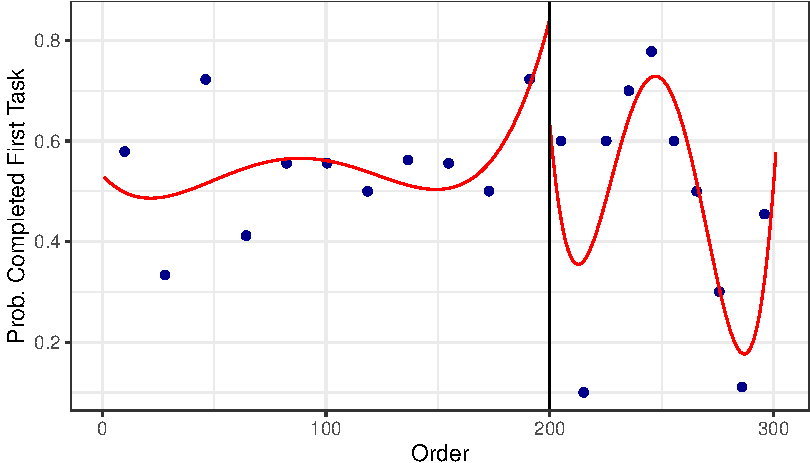
\includegraphics{The-Sources-of-Researcher-Variation-in-Economics_files/figure-pdf/fig-rdd-1.pdf}

}

\caption{\label{fig-rdd}Impact of Guaranteed Payment on Probability of
Task 1 Completion}

\end{figure}

Figure \ref{fig-rdd} shows no meaningful effect of being guaranteed
payment on the probability of completing Task 1. In additional results
in the appendix, using a linear regression specification of the
regression discontinuity design and the full range of the data (not
including the late sign-ups) to maximize statistical power,\footnote{Use
  of the full range, rather than a bandwidth, is justified given that
  the running variable is randomly assigned.} we again find no
statistically significant effect of being guaranteed treatment. This is
suggestive that participants were not simply signing up in an attempt to
get a \$2,000 payment for little effort.

\hypertarget{sample-characteristics}{%
\paragraph{Sample Characteristics}\label{sample-characteristics}}

Tables \ref{tab-samp1} to \ref{tab-samp3} show the characteristics of
the recruited sample, and how those characteristics changed with
eligibility and attrition. Task 2 is omitted as an attrition stage since
so few people dropped out between Task 1 and Task 2.

Table \ref{tab-samp1} shows that the majority of researchers were
recruited via social media, with only about 9\% coming from a department
email, 4\% from a professional organization email, and 9\% from some
other source (like word-of-mouth). Those recruited from another source
were less likely to qualify for the study, and slightly less likely to
finish, while those recruited from social media were most likely to
qualify and finish. We also asked researchers how certain they were of
their ability to finish the first task as well as the full set of tasks,
on a scale of 1 to 100. Enrollees were about 90\% confident in their
ability to complete the full set of research tasks (although only about
50\% did). Those who were more confident were slightly more likely to
actually finish, and average confidence rates of those who did finish
were about 92\% instead of 90\%.

\begin{table}[!htbp] \centering \renewcommand*{\arraystretch}{1.1}\caption{Researcher Recruitment Source and Completion Confidence}\label{tab-samp1}\resizebox{\textwidth}{!}{
\begin{tabular}{lrrrrrrrrrrrr}
\hline
\hline
Round & \multicolumn{3}{c}{Original signup} & \multicolumn{3}{c}{Assigned task 1} & \multicolumn{3}{c}{Finished task 1} & \multicolumn{3}{c}{Finished task 3}  \\ 
 Variable & \multicolumn{1}{c}{N} & \multicolumn{1}{c}{Mean} & \multicolumn{1}{c}{SD} & \multicolumn{1}{c}{N} & \multicolumn{1}{c}{Mean} & \multicolumn{1}{c}{SD} & \multicolumn{1}{c}{N} & \multicolumn{1}{c}{Mean} & \multicolumn{1}{c}{SD} & \multicolumn{1}{c}{N} & \multicolumn{1}{c}{Mean} & \multicolumn{1}{c}{SD} \\ 
\hline
Recruitment Source & 347 &  &  & 285 &  &  & 150 &  &  & 142 &  &  \\ 
... Social media & 270 & 78\% &  & 224 & 79\% &  & 124 & 83\% &  & 116 & 82\% &  \\ 
... Department email & 31 & 9\% &  & 28 & 10\% &  & 13 & 9\% &  & 13 & 9\% &  \\ 
... Email of a professional organization & 15 & 4\% &  & 10 & 4\% &  & 4 & 3\% &  & 4 & 3\% &  \\ 
... Other & 31 & 9\% &  & 23 & 8\% &  & 9 & 6\% &  & 9 & 6\% &  \\ 
Certainty to Finish Task 1 & 355 & 90 & 11 & 292 & 90 & 10 & 153 & 92 & 8.4 & 145 & 92 & 8.3 \\ 
Certainty to Finish Task 3 & 355 & 89 & 12 & 292 & 89 & 12 & 153 & 91 & 9.9 & 145 & 91 & 9.6\\ 
\hline
\hline
\end{tabular}
}
\end{table}

Table \ref{tab-samp1} shows the professional experience of enrollees.

While graduate students were considered eligible for the project as long
as they had a published or forthcoming paper, the great majority of
eligible researchers (83\%) had PhDs. PhD holders were also more likely
than other eligible researchers to complete all three tasks.

These PhDs are split across faculty (62\%) and other non-faculty
researchers (22\%), both of which were more likely than graduate
students to finish all three rounds. Note that the researchers in these
categories who do not hold PhDs were either people who had been hired to
faculty roles without holding PhDs (such as ABDs, or people in countries
where a faculty position requires only a Master's degree), or people
with Master's degrees in non-faculty research positions who had
published academic papers (some of whom were still graduate students).

Most of the researchers had at least one published paper, and
researchers with 6+ papers were more likely than others to complete all
three research tasks. Those with ``No Academic Papers'' are non-academic
researchers who produce work not intended for academic journal
publication. Those with ``No Published Academic Papers'' have papers
that are forthcoming, or are faculty who only have working papers and no
publications.

The set of researchers in the study generally do not work in the
specific subfield that the research task is in. The research task is
similar to many studies done across all of applied microeconomics, but
specifically is on the topics of labor and immigration. About a third of
the enrollees had done research in either immigration or labor
previously, and these researchers were somewhat more likely to complete
all three tasks. No researchers enrolled who had previously worked in
both immigration and labor.

\begin{table}[!htbp] \centering \renewcommand*{\arraystretch}{1.1}\caption{Researcher Professional Experience}\label{tab-samp2}\resizebox{\textwidth}{!}{
\begin{tabular}{lrrrrrrrr}
\hline
\hline
Round & \multicolumn{2}{c}{Original signup} & \multicolumn{2}{c}{Assigned task 1} & \multicolumn{2}{c}{Finished task 1} & \multicolumn{2}{c}{Finished task 3}  \\ 
 Variable & \multicolumn{1}{c}{N} & \multicolumn{1}{c}{Percent} & \multicolumn{1}{c}{N} & \multicolumn{1}{c}{Percent} & \multicolumn{1}{c}{N} & \multicolumn{1}{c}{Percent} & \multicolumn{1}{c}{N} & \multicolumn{1}{c}{Percent} \\ 
\hline
Degree & 360 &  & 295 &  & 154 &  & 146 &  \\ 
... No graduate school & 3 & 1\% & 0 & 0\% & 0 & 0\% & 0 & 0\% \\ 
... Some Grad School & 14 & 4\% & 5 & 2\% & 3 & 2\% & 2 & 1\% \\ 
... Master's degree & 78 & 22\% & 44 & 15\% & 17 & 11\% & 17 & 12\% \\ 
... Prof. Degree & 3 & 1\% & 1 & 0\% & 0 & 0\% & 0 & 0\% \\ 
... PhD & 262 & 73\% & 245 & 83\% & 134 & 87\% & 127 & 87\% \\ 
Occupation & 361 &  & 295 &  & 154 &  & 146 &  \\ 
... Faculty & 191 & 53\% & 182 & 62\% & 99 & 64\% & 98 & 67\% \\ 
... Grad. Student & 69 & 19\% & 36 & 12\% & 13 & 8\% & 12 & 8\% \\ 
... Other & 14 & 4\% & 11 & 4\% & 5 & 3\% & 3 & 2\% \\ 
... Other Researcher & 87 & 24\% & 66 & 22\% & 37 & 24\% & 33 & 23\% \\ 
Research Experience & 361 &  & 295 &  & 154 &  & 146 &  \\ 
... 1-5 Papers in Applied Micro & 162 & 45\% & 152 & 52\% & 74 & 48\% & 70 & 48\% \\ 
... 6+ Papers & 104 & 29\% & 102 & 35\% & 58 & 38\% & 57 & 39\% \\ 
... No Academic Papers & 17 & 5\% & 4 & 1\% & 3 & 2\% & 3 & 2\% \\ 
... No Published Academic Papers & 78 & 22\% & 37 & 13\% & 19 & 12\% & 16 & 11\% \\ 
Field & 333 &  & 270 &  & 145 &  & 138 &  \\ 
... Immigration \& Labor & 0 & 0\% & 0 & 0\% & 0 & 0\% & 0 & 0\% \\ 
... Immigration & 8 & 2\% & 6 & 2\% & 4 & 3\% & 4 & 3\% \\ 
... Labor & 102 & 31\% & 85 & 31\% & 49 & 34\% & 47 & 34\% \\ 
... Neither & 223 & 67\% & 179 & 66\% & 92 & 63\% & 87 & 63\%\\ 
\hline
\hline
\end{tabular}
}
\end{table}

Table \ref{tab-samp3} shows the demographics of the researcher sample.
The eligible sample was just under 80\% male and more than 55\% white,
and both percentages grew by the conclusion of task 3, with the white
share growing significantly to 66\%. The 80\% male figure is similar to
the share male found for faculty at a selected set of top economics
departments in 2017 by Lundberg and Stearns (2019), and among all
actively publishing economists in 2019 by Card et al. (2022). A small
share reported being LGBTQ+, and this share remained constant over all
rounds of the research tasks. An additional form of demographic
difference is geographic. About half of the sample was situated in the
United States, and about half was from another country.\footnote{Exact
  figures are not given for geography, and crosstabulations across
  geography are not given, because non-geographic demographic
  information comes from a survey where we acquired permission to share
  aggregate figures. Geographic information, on the other hand, comes
  from researcher payments information, for which we did not request
  permission to share responses.} The representativeness of the racial
mixture is difficult to assess for this reason; 66\% white would be low
if the entire sample were from the United States (Stansbury and Schultz
2023), but it is unclear what the population rate is in a 50\% US/50\%
other location sample.

\begin{table}[!htbp] \centering \renewcommand*{\arraystretch}{1.1}\caption{Researcher Demographics}\label{tab-samp3}\resizebox{\textwidth}{!}{
\begin{tabular}{lrrrrrrrr}
\hline
\hline
Round & \multicolumn{2}{c}{Original signup} & \multicolumn{2}{c}{Assigned task 1} & \multicolumn{2}{c}{Finished task 1} & \multicolumn{2}{c}{Finished task 3}  \\ 
 Variable & \multicolumn{1}{c}{N} & \multicolumn{1}{c}{Percent} & \multicolumn{1}{c}{N} & \multicolumn{1}{c}{Percent} & \multicolumn{1}{c}{N} & \multicolumn{1}{c}{Percent} & \multicolumn{1}{c}{N} & \multicolumn{1}{c}{Percent} \\ 
\hline
Gender & 359 &  & 294 &  & 154 &  & 146 &  \\ 
... Female & 81 & 23\% & 64 & 22\% & 28 & 18\% & 26 & 18\% \\ 
... Male & 274 & 76\% & 230 & 78\% & 126 & 82\% & 120 & 82\% \\ 
... Non-binary / third gender & 1 & 0\% & 0 & 0\% & 0 & 0\% & 0 & 0\% \\ 
... Prefer not to say & 3 & 1\% & 0 & 0\% & 0 & 0\% & 0 & 0\% \\ 
Race & 360 &  & 294 &  & 154 &  & 146 &  \\ 
... White & 188 & 52\% & 164 & 56\% & 100 & 65\% & 97 & 66\% \\ 
... Asian & 79 & 22\% & 60 & 20\% & 25 & 16\% & 25 & 17\% \\ 
... Black or African American & 27 & 8\% & 21 & 7\% & 4 & 3\% & 4 & 3\% \\ 
... Hispanic & 25 & 7\% & 19 & 6\% & 10 & 6\% & 9 & 6\% \\ 
... Other or Multiracial & 41 & 11\% & 30 & 10\% & 15 & 10\% & 11 & 8\% \\ 
LGBTQ+ & 360 &  & 294 &  & 154 &  & 146 &  \\ 
... Yes & 18 & 5\% & 14 & 5\% & 7 & 5\% & 7 & 5\% \\ 
... No & 323 & 90\% & 268 & 91\% & 137 & 89\% & 129 & 88\% \\ 
... Prefer not to say & 19 & 5\% & 12 & 4\% & 10 & 6\% & 10 & 7\%\\ 
\hline
\hline
\end{tabular}
}
\end{table}


One researcher did complete all three research tasks, and appears in the
above tables, but their work has been removed from the results that
follow in the rest of the paper, as due to a misunderstanding of the
instructions, their work did not attempt to estimate the effect of DACA
on the probability of employment.

As a whole, the goal of constructing a sample that largely reflects the
group of people who publish work in applied microeconomics. The sample
is skewed towards the United States, which is partially driven by the
emails sent to US economics departments, the fact that the project was
advertised and carried out in English, and the fact that the project
organizers are in the United States and advertised the project using
their own social media. Given that caveat, the makeup of the sample
appears to be fairly similar to the makeup of the profession itself,
although this is difficult to verify for some demographics.

\hypertarget{results}{%
\section{Results}\label{results}}

(move these around as appropriate; the recruitment and attrition stuff
might move up to data)

\hypertarget{variation-in-effects-and-sample-sizes}{%
\subsection{Variation in Effects and Sample
Sizes}\label{variation-in-effects-and-sample-sizes}}

\includegraphics{The-Sources-of-Researcher-Variation-in-Economics_files/figure-pdf/unnamed-chunk-11-1.pdf}

\includegraphics{The-Sources-of-Researcher-Variation-in-Economics_files/figure-pdf/unnamed-chunk-12-1.pdf}

\includegraphics{The-Sources-of-Researcher-Variation-in-Economics_files/figure-pdf/unnamed-chunk-13-1.pdf}

\includegraphics{The-Sources-of-Researcher-Variation-in-Economics_files/figure-pdf/unnamed-chunk-14-1.pdf}


\hypertarget{researcher-characteristics-and-effects}{%
\subsection{Researcher Characteristics and
Effects}\label{researcher-characteristics-and-effects}}

\begin{longtable}[]{@{}
  >{\raggedright\arraybackslash}p{(\columnwidth - 18\tabcolsep) * \real{0.2703}}
  >{\raggedright\arraybackslash}p{(\columnwidth - 18\tabcolsep) * \real{0.0811}}
  >{\raggedright\arraybackslash}p{(\columnwidth - 18\tabcolsep) * \real{0.0811}}
  >{\raggedright\arraybackslash}p{(\columnwidth - 18\tabcolsep) * \real{0.0811}}
  >{\raggedright\arraybackslash}p{(\columnwidth - 18\tabcolsep) * \real{0.0811}}
  >{\raggedright\arraybackslash}p{(\columnwidth - 18\tabcolsep) * \real{0.0811}}
  >{\raggedright\arraybackslash}p{(\columnwidth - 18\tabcolsep) * \real{0.0811}}
  >{\raggedright\arraybackslash}p{(\columnwidth - 18\tabcolsep) * \real{0.0811}}
  >{\raggedright\arraybackslash}p{(\columnwidth - 18\tabcolsep) * \real{0.0811}}
  >{\raggedright\arraybackslash}p{(\columnwidth - 18\tabcolsep) * \real{0.0811}}@{}}
\toprule\noalign{}
\begin{minipage}[b]{\linewidth}\raggedright
Predictor
\end{minipage} & \begin{minipage}[b]{\linewidth}\raggedright
R1: F
\end{minipage} & \begin{minipage}[b]{\linewidth}\raggedright
p
\end{minipage} & \begin{minipage}[b]{\linewidth}\raggedright
R2
\end{minipage} & \begin{minipage}[b]{\linewidth}\raggedright
R2: F
\end{minipage} & \begin{minipage}[b]{\linewidth}\raggedright
p
\end{minipage} & \begin{minipage}[b]{\linewidth}\raggedright
R2
\end{minipage} & \begin{minipage}[b]{\linewidth}\raggedright
R3: F
\end{minipage} & \begin{minipage}[b]{\linewidth}\raggedright
p
\end{minipage} & \begin{minipage}[b]{\linewidth}\raggedright
R2
\end{minipage} \\
\midrule\noalign{}
\endhead
\bottomrule\noalign{}
\endlastfoot
Degree & 0.929 & 0.337 & 0.007 & 0.122 & 0.727 & 0.001 & 0.085 & 0.771 &
0.001 \\
Occupation & 1.195 & 0.316 & 0.034 & 0.453 & 0.770 & 0.013 & 2.501 &
0.045 & 0.068 \\
Research Experience & 1.080 & 0.342 & 0.015 & 0.370 & 0.692 & 0.005 &
0.416 & 0.660 & 0.006 \\
Gender & 0.161 & 0.689 & 0.001 & 0.255 & 0.614 & 0.002 & 1.364 & 0.245 &
0.009 \\
Race & 1.026 & 0.383 & 0.022 & 1.306 & 0.275 & 0.028 & 0.342 & 0.795 &
0.007 \\
LGBTQ+ & 0.426 & 0.654 & 0.006 & 0.183 & 0.833 & 0.003 & 0.045 & 0.956 &
0.001 \\
Recruitment Source & 0.360 & 0.698 & 0.005 & 1.661 & 0.194 & 0.024 &
1.400 & 0.250 & 0.020 \\
Field & 1.406 & 0.238 & 0.011 & 4.562 & 0.035 & 0.034 & 0.831 & 0.364 &
0.006 \\
Coding Language & 3.861 & 0.051 & 0.027 & 3.117 & 0.080 & 0.022 & 0.653
& 0.420 & 0.005 \\
\end{longtable}

\begin{longtable}[]{@{}
  >{\raggedright\arraybackslash}p{(\columnwidth - 18\tabcolsep) * \real{0.2703}}
  >{\raggedright\arraybackslash}p{(\columnwidth - 18\tabcolsep) * \real{0.0811}}
  >{\raggedright\arraybackslash}p{(\columnwidth - 18\tabcolsep) * \real{0.0811}}
  >{\raggedright\arraybackslash}p{(\columnwidth - 18\tabcolsep) * \real{0.0811}}
  >{\raggedright\arraybackslash}p{(\columnwidth - 18\tabcolsep) * \real{0.0811}}
  >{\raggedright\arraybackslash}p{(\columnwidth - 18\tabcolsep) * \real{0.0811}}
  >{\raggedright\arraybackslash}p{(\columnwidth - 18\tabcolsep) * \real{0.0811}}
  >{\raggedright\arraybackslash}p{(\columnwidth - 18\tabcolsep) * \real{0.0811}}
  >{\raggedright\arraybackslash}p{(\columnwidth - 18\tabcolsep) * \real{0.0811}}
  >{\raggedright\arraybackslash}p{(\columnwidth - 18\tabcolsep) * \real{0.0811}}@{}}
\toprule\noalign{}
\begin{minipage}[b]{\linewidth}\raggedright
Predictor
\end{minipage} & \begin{minipage}[b]{\linewidth}\raggedright
R1: F
\end{minipage} & \begin{minipage}[b]{\linewidth}\raggedright
p
\end{minipage} & \begin{minipage}[b]{\linewidth}\raggedright
R2
\end{minipage} & \begin{minipage}[b]{\linewidth}\raggedright
R2: F
\end{minipage} & \begin{minipage}[b]{\linewidth}\raggedright
p
\end{minipage} & \begin{minipage}[b]{\linewidth}\raggedright
R2
\end{minipage} & \begin{minipage}[b]{\linewidth}\raggedright
R3: F
\end{minipage} & \begin{minipage}[b]{\linewidth}\raggedright
p
\end{minipage} & \begin{minipage}[b]{\linewidth}\raggedright
R2
\end{minipage} \\
\midrule\noalign{}
\endhead
\bottomrule\noalign{}
\endlastfoot
Degree & 1.915 & 0.169 & 0.013 & 0.740 & 0.391 & 0.005 & 0.630 & 0.429 &
0.004 \\
Occupation & 0.890 & 0.472 & 0.025 & 0.535 & 0.710 & 0.015 & 1.845 &
0.124 & 0.051 \\
Research Experience & 1.364 & 0.259 & 0.019 & 0.284 & 0.754 & 0.004 &
0.741 & 0.478 & 0.011 \\
Gender & 1.576 & 0.211 & 0.011 & 1.102 & 0.296 & 0.008 & 0.144 & 0.705 &
0.001 \\
Race & 2.180 & 0.093 & 0.045 & 0.129 & 0.943 & 0.003 & 0.762 & 0.517 &
0.016 \\
LGBTQ+ & 0.202 & 0.817 & 0.003 & 0.515 & 0.599 & 0.007 & 0.253 & 0.776 &
0.004 \\
Recruitment Source & 2.064 & 0.131 & 0.030 & 0.197 & 0.822 & 0.003 &
0.552 & 0.577 & 0.008 \\
Field & 0.077 & 0.781 & 0.001 & 0.936 & 0.335 & 0.007 & 0.072 & 0.789 &
0.001 \\
Coding Language & 4.369 & 0.038 & 0.030 & 4.537 & 0.035 & 0.032 & 5.022
& 0.027 & 0.035 \\
\end{longtable}

\includegraphics{The-Sources-of-Researcher-Variation-in-Economics_files/figure-pdf/unnamed-chunk-17-1.pdf}


\hypertarget{peer-review}{%
\subsection{Peer Review}\label{peer-review}}

\includegraphics{The-Sources-of-Researcher-Variation-in-Economics_files/figure-pdf/unnamed-chunk-18-1.pdf}

\hypertarget{do-you-become-more-like-your-reviewer}{%
\subsubsection{Do You Become More Like Your
Reviewer?}\label{do-you-become-more-like-your-reviewer}}

\includegraphics{The-Sources-of-Researcher-Variation-in-Economics_files/figure-pdf/unnamed-chunk-19-1.pdf}

\begin{table}
\centering
\begin{tabular}[t]{lcc}
\toprule
  & sample: Task 1 & sample: Task 2\\
\midrule

(Intercept) & \num{0.088}*** & \num{0.063}***\\
 & (\num{0.009}) & \vphantom{1} (\num{0.009})\\
ComparisonNext Round & \num{-0.029}** & \num{-0.006}\\
 & (\num{0.013}) & \vphantom{2} (\num{0.013})\\
ComparisonNext vs. This & \num{-0.018} & \num{0.001}\\
 & (\num{0.013}) & \vphantom{1} (\num{0.013})\\
TypeUnreviewed & \num{-0.047}*** & \num{-0.001}\\
 & (\num{0.009}) & (\num{0.009})\\
ComparisonNext Round × TypeUnreviewed & \num{0.051}*** & \num{-0.029}**\\
 & (\num{0.014}) & (\num{0.013})\\
ComparisonNext vs. This × TypeUnreviewed & \num{0.029}** & \num{-0.016}\\
 & (\num{0.013}) & (\num{0.013})\\
\midrule
Num.Obs. & \num{7266} & \num{6964}\\

\bottomrule
\multicolumn{3}{l}{\rule{0pt}{1em}* p $<$ 0.1, ** p $<$ 0.05, *** p $<$ 0.01}\\
\end{tabular}
\end{table}

TO DO: The same but for sample sizes and analytic choices

\hypertarget{analytic-choices}{%
\subsection{Analytic Choices}\label{analytic-choices}}

\begin{table}

\caption{}
\centering
\begin{tabular}[t]{llllll}
\toprule
Variable & N & Percent & Variable & N & Percent\\
\midrule
Method & 437 &  & S.E. Adjustment & 438 & \\
... Linear Regression & 358 & 82\% & ... Cluster (State) & 118 & 27\%\\
... Logit/Probit & 57 & 13\% & ... Cluster (State \& Year) & 58 & 13\%\\
... Matching & 11 & 3\% & ... Cluster (ID/Strata/Other) & 65 & 15\%\\
... New DID Estimator & 7 & 2\% & ... Het-Robust & 76 & 17\%\\
\addlinespace
... Other & 4 & 1\% & ... Other/Bootstrap & 23 & 5\%\\
Weights & 438 &  & ... None & 98 & 22\%\\
... No Sample Weights & 329 & 75\% &  &  & \\
... Sample Weights & 109 & 25\% &  &  & \\
\bottomrule
\multicolumn{6}{l}{\textsuperscript{} This table shows details on estimation, not research design.}\\
\multicolumn{6}{l}{"Difference-in-differences" implemented with linear regression, for example, counts}\\
\multicolumn{6}{l}{here as linear regression.}\\
\end{tabular}
\end{table}

\hypertarget{sample-limitations}{%
\subsection{Sample Limitations}\label{sample-limitations}}

\begin{table}

\caption{Summary Statistics}
\centering
\begin{tabular}[t]{lllllllll}
\toprule
Variable & N & Mean & Std. Dev. & Min & Pctl. 25 & Pctl. 50 & Pctl. 75 & Max\\
\midrule
Round: Task 1 &  &  &  &  &  &  &  & \\
Whole Sample & 146 & 4.8 & 2.8 & 0 & 3 & 5 & 6 & 14\\
Treated Group & 146 & 8.1 & 2.7 & 1 & 7 & 8 & 10 & 15\\
Untreated Group & 146 & 7.4 & 3.2 & 1 & 5.2 & 8 & 10 & 15\\
Round: Task 2 &  &  &  &  &  &  &  & \\
\addlinespace
Whole Sample & 146 & 6.5 & 4 & 0 & 3 & 7 & 9 & 15\\
Treated Group & 146 & 9.4 & 3.5 & 1 & 8 & 10 & 12 & 16\\
Untreated Group & 146 & 9.5 & 3.3 & 1 & 8 & 10 & 12 & 16\\
\bottomrule
\end{tabular}
\end{table}

\begin{table}[!htbp] \centering \renewcommand*{\arraystretch}{1.1}\caption{Sample Restriction Methods}\resizebox{.9\textwidth}{!}{
\begin{tabular}{lrrrrrrrr}
\hline
\hline
Round/Sample & \multicolumn{2}{c}{Task 1 All} & \multicolumn{2}{c}{Task 1 Treated} & \multicolumn{2}{c}{Task 2 All} & \multicolumn{2}{c}{Task 2 Treated}  \\ 
 Variable & \multicolumn{1}{c}{N} & \multicolumn{1}{c}{Percent} & \multicolumn{1}{c}{N} & \multicolumn{1}{c}{Percent} & \multicolumn{1}{c}{N} & \multicolumn{1}{c}{Percent} & \multicolumn{1}{c}{N} & \multicolumn{1}{c}{Percent} \\ 
\hline
Hispanic & 142 &  & 135 &  & 137 &  & 131 &  \\ 
... Hispanic-Mexican & 91 & 64\% & 98 & 73\% & 96 & 70\% & 101 & 77\% \\ 
... Hispanic-Any & 7 & 5\% & 8 & 6\% & 7 & 5\% & 8 & 6\% \\ 
... Hispanic-Mex or Mex-Born & 5 & 4\% & 6 & 4\% & 0 & 0\% & 1 & 1\% \\ 
... Multistep Condition & 2 & 1\% & 2 & 1\% & 1 & 1\% & 1 & 1\% \\ 
... None & 37 & 26\% & 21 & 16\% & 33 & 24\% & 20 & 15\% \\ 
Birthplace & 142 &  & 135 &  & 137 &  & 131 &  \\ 
... Mexican-Born & 89 & 63\% & 83 & 61\% & 91 & 66\% & 88 & 67\% \\ 
... Hispanic-Mex or Mex-Born & 4 & 3\% & 2 & 1\% & 0 & 0\% & 1 & 1\% \\ 
... Non-US Born & 1 & 1\% & 1 & 1\% & 3 & 2\% & 0 & 0\% \\ 
... Central America-Born & 1 & 1\% & 1 & 1\% & 1 & 1\% & 1 & 1\% \\ 
... None & 47 & 33\% & 48 & 36\% & 42 & 31\% & 41 & 31\% \\ 
Citizenship & 142 &  & 135 &  & 137 &  & 131 &  \\ 
... Non-Citizen & 70 & 49\% & 100 & 74\% & 85 & 62\% & 107 & 82\% \\ 
... Foreign-Born & 3 & 2\% & 3 & 2\% & 1 & 1\% & 0 & 0\% \\ 
... Non-Cit or Natlzd post-2012 & 1 & 1\% & 4 & 3\% & 2 & 1\% & 4 & 3\% \\ 
... Citizen (various) & 1 & 1\% & 3 & 2\% & 1 & 1\% & 2 & 2\% \\ 
... Multistep Condition & 2 & 1\% & 1 & 1\% & 0 & 0\% & 0 & 0\% \\ 
... Other & 7 & 5\% & 9 & 7\% & 3 & 2\% & 6 & 5\% \\ 
... None & 58 & 41\% & 15 & 11\% & 45 & 33\% & 12 & 9\% \\ 
Age at Migration & 142 &  & 135 &  & 137 &  & 131 &  \\ 
... < 16 & 12 & 8\% & 81 & 60\% & 50 & 36\% & 90 & 69\% \\ 
... <= 16 & 4 & 3\% & 15 & 11\% & 7 & 5\% & 12 & 9\% \\ 
... > 16 & 0 & 0\% & 1 & 1\% & 0 & 0\% & 0 & 0\% \\ 
... Any Age & 1 & 1\% & 0 & 0\% & 0 & 0\% & 0 & 0\% \\ 
... Multistep Condition & 1 & 1\% & 0 & 0\% & 0 & 0\% & 0 & 0\% \\ 
... Other & 26 & 18\% & 23 & 17\% & 11 & 8\% & 13 & 10\% \\ 
... None & 98 & 69\% & 15 & 11\% & 69 & 50\% & 16 & 12\% \\ 
Age in June 2012 & 146 &  & 146 &  & 146 &  & 146 &  \\ 
... Year-Quarter Age & 23 & 16\% & 114 & 78\% & 75 & 51\% & 116 & 79\% \\ 
... Year-Only Age & 12 & 8\% & 7 & 5\% & 9 & 6\% & 10 & 7\% \\ 
... None & 111 & 76\% & 25 & 17\% & 62 & 42\% & 20 & 14\% \\ 
Year of Immigration & 142 &  & 135 &  & 137 &  & 131 &  \\ 
... < 2007 & 11 & 8\% & 38 & 28\% & 30 & 22\% & 42 & 32\% \\ 
... <= 2007 & 9 & 6\% & 46 & 34\% & 22 & 16\% & 39 & 30\% \\ 
... < 2012 & 2 & 1\% & 0 & 0\% & 0 & 0\% & 2 & 2\% \\ 
... <= 2012 & 2 & 1\% & 2 & 1\% & 1 & 1\% & 3 & 2\% \\ 
... >= 2007 & 1 & 1\% & 1 & 1\% & 0 & 0\% & 0 & 0\% \\ 
... Any Year & 7 & 5\% & 3 & 2\% & 2 & 1\% & 1 & 1\% \\ 
... Multistep Condition & 2 & 1\% & 1 & 1\% & 0 & 0\% & 2 & 2\% \\ 
... Other & 4 & 3\% & 2 & 1\% & 2 & 1\% & 1 & 1\% \\ 
... None & 104 & 73\% & 42 & 31\% & 80 & 58\% & 41 & 31\% \\ 
Education/Veteran & 146 &  & 146 &  & 146 &  & 146 &  \\ 
... HS Grad or Veteran & 0 & 0\% & 2 & 1\% & 66 & 45\% & 96 & 66\% \\ 
... 12th Grade or Veteran & 0 & 0\% & 0 & 0\% & 2 & 1\% & 4 & 3\% \\ 
... HS Grad & 14 & 10\% & 14 & 10\% & 4 & 3\% & 6 & 4\% \\ 
... HS Grad or In School & 0 & 0\% & 0 & 0\% & 0 & 0\% & 0 & 0\% \\ 
... HS Grad or Non-Veteran & 0 & 0\% & 0 & 0\% & 3 & 2\% & 4 & 3\% \\ 
... Other & 5 & 3\% & 10 & 7\% & 7 & 5\% & 12 & 8\% \\ 
... None & 127 & 87\% & 120 & 82\% & 64 & 44\% & 24 & 16\% \\ 
Years Continuous in USA & 146 &  & 146 &  & 146 &  & 146 &  \\ 
... Used YRSUSA & 9 & 6\% & 40 & 27\% & 17 & 12\% & 40 & 27\% \\ 
... No YRSUSA & 137 & 94\% & 106 & 73\% & 129 & 88\% & 106 & 73\%\\ 
\hline
\hline
\end{tabular}
}
\end{table}

\begin{table}[!htbp] \centering \renewcommand*{\arraystretch}{1.1}\caption{Task 1 Effect and Samples by Sample Definitions}\resizebox{\textwidth}{!}{
\begin{tabular}{llllllllll}
\hline
\hline
 & \multicolumn{3}{c}{Treated-Group Restriction} & \multicolumn{6}{c}{All-Sample Restriction}  \\ 
 Variable & Effect Pctl. 25 & Pctl. 50 & Pctl. 75 & Effect Pctl. 25 & Pctl. 50 & Pctl. 75 & Samp Size Pctl. 25 & Pctl. 50 & Pctl. 75 \\ 
\hline
Hispanic &  &  &  &  &  &  &  &  &  \\ 
... Hispanic-Mexican & 0.014 & 0.032 & 0.054 & 0.015 & 0.032 & 0.055 & 69,522 & 173,803 & 295,926 \\ 
... Hispanic-Any & 0.030 & 0.037 & 0.050 & 0.030 & 0.045 & 0.054 & 24,276 & 109,759 & 166,270 \\ 
... Hispanic-Mex or Mex-Born & 0.018 & 0.021 & 0.026 & 0.021 & 0.022 & 0.027 & 51,754 & 127,504 & 179,960 \\ 
... Multistep Condition & -0.009 & 0.001 & 0.010 & -0.009 & 0.001 & 0.010 & 326,913 & 366,804 & 406,696 \\ 
... None & 0.017 & 0.023 & 0.052 & 0.013 & 0.026 & 0.051 & 75,698 & 263,527 & 808,057 \\ 
Birthplace &  &  &  &  &  &  &  &  &  \\ 
... Mexican-Born & 0.016 & 0.030 & 0.048 & 0.016 & 0.030 & 0.050 & 61,600 & 143,738 & 277,264 \\ 
... Hispanic-Mex or Mex-Born & 0.041 & 0.100 & 0.160 & 0.004 & 0.016 & 0.070 & 215,436 & 289,311 & 330,348 \\ 
... Non-US Born & -0.020 & -0.020 & -0.020 & -0.020 & -0.020 & -0.020 & 110,273 & 110,273 & 110,273 \\ 
... Central America-Born & 0.057 & 0.057 & 0.057 & 0.057 & 0.057 & 0.057 & 9,711 & 9,711 & 9,711 \\ 
... None & 0.015 & 0.033 & 0.054 & 0.014 & 0.036 & 0.053 & 78,426 & 277,277 & 746,663 \\ 
Citizenship &  &  &  &  &  &  &  &  &  \\ 
... Non-Citizen & 0.018 & 0.030 & 0.052 & 0.022 & 0.035 & 0.056 & 67,068 & 142,792 & 277,274 \\ 
... Foreign-Born & 0.026 & 0.037 & 0.180 & 0.026 & 0.037 & 0.180 & 341,338 & 586,271 & 605,241 \\ 
... Non-Cit or Natlzd post-2012 & 0.001 & 0.022 & 0.028 & 0.017 & 0.017 & 0.017 & 13,377 & 13,377 & 13,377 \\ 
... Citizen (various) & 0.019 & 0.023 & 0.047 & 0.015 & 0.015 & 0.015 & 268,238 & 268,238 & 268,238 \\ 
... Multistep Condition & 0.009 & 0.009 & 0.009 & -0.034 & -0.020 & -0.005 & 899,372 & 1,694,116 & 2,488,861 \\ 
... Other & 0.023 & 0.041 & 0.053 & 0.023 & 0.037 & 0.046 & 13,427 & 17,759 & 84,944 \\ 
... None & 0.009 & 0.028 & 0.052 & 0.011 & 0.021 & 0.043 & 91,829 & 242,029 & 675,566 \\ 
Age at Migration &  &  &  &  &  &  &  &  &  \\ 
... < 16 & 0.017 & 0.030 & 0.051 & 0.018 & 0.026 & 0.046 & 28,348 & 44,288 & 119,180 \\ 
... <= 16 & 0.011 & 0.022 & 0.049 & 0.039 & 0.042 & 0.163 & 93,442 & 162,585 & 224,645 \\ 
... > 16 & 0.060 & 0.060 & 0.060 &  &  &  &  &  &  \\ 
... Any Age &  &  &  & -0.019 & -0.019 & -0.019 & 287,021 & 287,021 & 287,021 \\ 
... Multistep Condition &  &  &  & 0.009 & 0.009 & 0.009 & 104,628 & 104,628 & 104,628 \\ 
... Other & 0.018 & 0.032 & 0.054 & 0.018 & 0.032 & 0.057 & 34,870 & 117,257 & 202,525 \\ 
... None & 0.000 & 0.028 & 0.050 & 0.013 & 0.030 & 0.052 & 99,873 & 255,769 & 507,856 \\ 
Age in June 2012 &  &  &  &  &  &  &  &  &  \\ 
... Year-Quarter Age & 0.016 & 0.030 & 0.052 & 0.018 & 0.037 & 0.051 & 40,586 & 132,637 & 297,176 \\ 
... Year-Only Age & 0.009 & 0.030 & 0.040 & 0.018 & 0.038 & 0.055 & 15,386 & 47,107 & 154,298 \\ 
... None & 0.012 & 0.027 & 0.036 & 0.014 & 0.029 & 0.051 & 83,418 & 205,147 & 424,859 \\ 
Year of Immigration &  &  &  &  &  &  &  &  &  \\ 
... < 2007 & 0.020 & 0.036 & 0.054 & 0.014 & 0.028 & 0.034 & 13,586 & 31,878 & 51,571 \\ 
... <= 2007 & 0.016 & 0.032 & 0.054 & 0.016 & 0.019 & 0.041 & 35,144 & 44,503 & 206,266 \\ 
... < 2012 &  &  &  & 0.039 & 0.051 & 0.064 & 88,982 & 103,534 & 118,086 \\ 
... <= 2012 & 0.042 & 0.118 & 0.194 & 0.029 & 0.092 & 0.155 & 263,220 & 471,364 & 679,507 \\ 
... >= 2007 & 0.012 & 0.012 & 0.012 & 0.012 & 0.012 & 0.012 & 245,635 & 245,635 & 245,635 \\ 
... Any Year & 0.018 & 0.030 & 0.040 & 0.021 & 0.034 & 0.044 & 31,170 & 116,405 & 212,998 \\ 
... Multistep Condition & 0.014 & 0.014 & 0.014 & 0.010 & 0.012 & 0.013 & 137,786 & 170,943 & 204,100 \\ 
... Other & 0.071 & 0.160 & 0.250 & 0.014 & 0.027 & 0.040 & 119,964 & 239,081 & 365,610 \\ 
... None & 0.016 & 0.028 & 0.043 & 0.016 & 0.032 & 0.053 & 110,144 & 230,665 & 474,472 \\ 
Education/Veteran &  &  &  &  &  &  &  &  &  \\ 
... HS Grad or Veteran & 0.043 & 0.065 & 0.088 &  &  &  &  &  &  \\ 
... HS Grad & 0.016 & 0.038 & 0.052 & 0.016 & 0.037 & 0.052 & 66,766 & 132,990 & 169,327 \\ 
... Other & 0.019 & 0.027 & 0.061 & 0.027 & 0.057 & 0.062 & 32,606 & 74,431 & 188,802 \\ 
... None & 0.014 & 0.030 & 0.051 & 0.014 & 0.029 & 0.051 & 63,107 & 204,239 & 397,308 \\ 
Years Continuous in USA &  &  &  &  &  &  &  &  &  \\ 
... Used YRSUSA & 0.017 & 0.029 & 0.053 & 0.019 & 0.025 & 0.050 & 35,144 & 118,438 & 155,898 \\ 
... No YRSUSA & 0.013 & 0.030 & 0.049 & 0.014 & 0.030 & 0.051 & 64,614 & 194,349 & 374,548\\ 
\hline
\hline
\end{tabular}
}
\end{table}

\begin{table}[!htbp] \centering \renewcommand*{\arraystretch}{1.1}\caption{Task 2 Effect and Samples by Sample Definitions}\resizebox{\textwidth}{!}{
\begin{tabular}{llllllllll}
\hline
\hline
 & \multicolumn{3}{c}{Treated-Group Restriction} & \multicolumn{6}{c}{All-Sample Restriction}  \\ 
 Variable & Effect Pctl. 25 & Pctl. 50 & Pctl. 75 & Effect Pctl. 25 & Pctl. 50 & Pctl. 75 & Samp Size Pctl. 25 & Pctl. 50 & Pctl. 75 \\ 
\hline
Hispanic &  &  &  &  &  &  &  &  &  \\ 
... Hispanic-Mexican & 0.018 & 0.033 & 0.058 & 0.017 & 0.030 & 0.057 & 18,680 & 25,056 & 38,154 \\ 
... Hispanic-Any & 0.028 & 0.050 & 0.063 & 0.024 & 0.042 & 0.058 & 22,983 & 24,011 & 25,568 \\ 
... Hispanic-Mex or Mex-Born & 0.048 & 0.048 & 0.048 &  &  &  &  &  &  \\ 
... Multistep Condition & 0.025 & 0.025 & 0.025 & 0.025 & 0.025 & 0.025 & 44,805 & 44,805 & 44,805 \\ 
... None & 0.024 & 0.043 & 0.062 & 0.026 & 0.045 & 0.074 & 19,236 & 27,531 & 61,340 \\ 
Birthplace &  &  &  &  &  &  &  &  &  \\ 
... Mexican-Born & 0.018 & 0.033 & 0.056 & 0.018 & 0.032 & 0.056 & 19,074 & 24,979 & 31,730 \\ 
... Hispanic-Mex or Mex-Born & 0.070 & 0.070 & 0.070 &  &  &  &  &  &  \\ 
... Non-US Born &  &  &  & 0.028 & 0.045 & 0.058 & 25,498 & 26,138 & 47,180 \\ 
... Central America-Born & 0.067 & 0.067 & 0.067 & 0.067 & 0.067 & 0.067 & 25,538 & 25,538 & 25,538 \\ 
... None & 0.018 & 0.040 & 0.074 & 0.018 & 0.040 & 0.070 & 18,750 & 25,639 & 72,235 \\ 
Citizenship &  &  &  &  &  &  &  &  &  \\ 
... Non-Citizen & 0.019 & 0.034 & 0.059 & 0.019 & 0.033 & 0.058 & 18,803 & 24,979 & 40,649 \\ 
... Foreign-Born &  &  &  & 0.004 & 0.004 & 0.004 & 164,135 & 164,135 & 164,135 \\ 
... Non-Cit or Natlzd post-2012 & 0.029 & 0.041 & 0.050 & 0.019 & 0.024 & 0.029 & 18,162 & 21,823 & 25,484 \\ 
... Citizen (various) & 0.014 & 0.024 & 0.035 & 0.045 & 0.045 & 0.045 & 19,168 & 19,168 & 19,168 \\ 
... Other & 0.040 & 0.054 & 0.060 & 0.031 & 0.059 & 0.059 & 21,828 & 24,011 & 90,368 \\ 
... None & 0.004 & 0.032 & 0.049 & 0.018 & 0.037 & 0.058 & 19,733 & 27,374 & 73,027 \\ 
Age at Migration &  &  &  &  &  &  &  &  &  \\ 
... < 16 & 0.018 & 0.035 & 0.057 & 0.028 & 0.041 & 0.059 & 19,246 & 23,350 & 27,134 \\ 
... <= 16 & 0.009 & 0.022 & 0.050 & 0.014 & 0.020 & 0.038 & 20,392 & 25,199 & 26,267 \\ 
... Other & 0.019 & 0.045 & 0.077 & 0.029 & 0.037 & 0.056 & 16,308 & 23,364 & 34,586 \\ 
... None & 0.028 & 0.045 & 0.066 & 0.015 & 0.028 & 0.057 & 19,270 & 30,416 & 97,507 \\ 
Age in June 2012 &  &  &  &  &  &  &  &  &  \\ 
... Year-Quarter Age & 0.021 & 0.037 & 0.058 & 0.024 & 0.037 & 0.057 & 19,562 & 25,199 & 41,156 \\ 
... Year-Only Age & 0.006 & 0.018 & 0.050 & 0.015 & 0.019 & 0.048 & 16,542 & 26,396 & 29,146 \\ 
... None & 0.007 & 0.016 & 0.024 & 0.006 & 0.025 & 0.059 & 18,803 & 25,414 & 86,316 \\ 
Year of Immigration &  &  &  &  &  &  &  &  &  \\ 
... < 2007 & 0.016 & 0.028 & 0.048 & 0.017 & 0.029 & 0.053 & 22,840 & 25,056 & 28,602 \\ 
... <= 2007 & 0.023 & 0.045 & 0.058 & 0.030 & 0.040 & 0.067 & 19,506 & 25,588 & 28,510 \\ 
... < 2012 & 0.038 & 0.047 & 0.055 &  &  &  &  &  &  \\ 
... <= 2012 & -0.011 & 0.068 & 0.290 & 0.068 & 0.068 & 0.068 & 6,600 & 6,600 & 6,600 \\ 
... Any Year & 0.059 & 0.059 & 0.059 & 0.049 & 0.052 & 0.056 & 18,409 & 20,276 & 22,144 \\ 
... Multistep Condition & 0.000 & 0.017 & 0.035 &  &  &  &  &  &  \\ 
... Other & 0.850 & 0.850 & 0.850 & 0.024 & 0.026 & 0.028 & 25,048 & 35,419 & 45,790 \\ 
... None & 0.018 & 0.037 & 0.058 & 0.015 & 0.034 & 0.057 & 18,776 & 25,418 & 70,229 \\ 
Education/Veteran &  &  &  &  &  &  &  &  &  \\ 
... HS Grad or Veteran & 0.018 & 0.034 & 0.058 & 0.018 & 0.035 & 0.058 & 18,814 & 23,690 & 27,641 \\ 
... 12th Grade or Veteran & 0.049 & 0.067 & 0.091 & 0.061 & 0.067 & 0.073 & 25,473 & 25,532 & 25,590 \\ 
... HS Grad & 0.025 & 0.047 & 0.057 & 0.035 & 0.047 & 0.055 & 15,036 & 18,260 & 23,155 \\ 
... HS Grad or Non-Veteran & 0.042 & 0.049 & 0.051 & 0.037 & 0.047 & 0.058 & 20,395 & 24,979 & 32,814 \\ 
... Other & 0.019 & 0.030 & 0.051 & 0.029 & 0.038 & 0.063 & 21,746 & 25,538 & 43,744 \\ 
... None & 0.005 & 0.017 & 0.051 & 0.007 & 0.025 & 0.052 & 19,750 & 37,323 & 138,560 \\ 
Years Continuous in USA &  &  &  &  &  &  &  &  &  \\ 
... Used YRSUSA & 0.017 & 0.038 & 0.061 & 0.029 & 0.035 & 0.064 & 15,252 & 22,833 & 25,199 \\ 
... No YRSUSA & 0.015 & 0.028 & 0.057 & 0.015 & 0.029 & 0.057 & 19,317 & 25,868 & 54,080\\ 
\hline
\hline
\end{tabular}
}
\end{table}

\hypertarget{control-variables}{%
\subsection{Control Variables}\label{control-variables}}

\begin{longtable}[]{@{}lrlll@{}}
\toprule\noalign{}
Control & N & Effect & Mean SE & Effect SD \\
\midrule\noalign{}
\endhead
\bottomrule\noalign{}
\endlastfoot
YRSUSA1 & 55 & 0.054 & 0.035 & 0.123 \\
AGE & 248 & 0.048 & 0.025 & 0.094 \\
YRIMMIG & 55 & 0.048 & 0.033 & 0.112 \\
MARST & 51 & 0.047 & 0.016 & 0.071 \\
SEX & 289 & 0.046 & 0.027 & 0.101 \\
STATE & 275 & 0.045 & 0.025 & 0.089 \\
AGE\_AT\_MIGRATION & 67 & 0.045 & 0.022 & 0.067 \\
YEAR & 267 & 0.045 & 0.026 & 0.094 \\
EDUC & 216 & 0.042 & 0.017 & 0.061 \\
None & 40 & 0.041 & 0.044 & 0.114 \\
OTHER & 278 & 0.040 & 0.038 & 0.086 \\
AGE\_IN\_2012 & 24 & 0.037 & 0.026 & 0.042 \\
STATEPOLICY & 99 & 0.037 & 0.033 & 0.108 \\
UNEMP & 128 & 0.036 & 0.033 & 0.097 \\
LFPR & 86 & 0.035 & 0.041 & 0.115 \\
SPEAKENG & 82 & 0.034 & 0.046 & 0.100 \\
RACE & 106 & 0.031 & 0.032 & 0.092 \\
\end{longtable}

\begin{longtable}[]{@{}llrlll@{}}
\toprule\noalign{}
Category & Control & N & Effect & Mean SE & Effect SD \\
\midrule\noalign{}
\endhead
\bottomrule\noalign{}
\endlastfoot
AGE & Linear Age & 164 & 0.058 & 0.024 & 0.107 \\
AGE & Age FE & 36 & 0.024 & 0.040 & 0.022 \\
AGE & Age Quadratic & 33 & 0.035 & 0.015 & 0.089 \\
EDUC & Linear Education & 122 & 0.040 & 0.016 & 0.066 \\
EDUC & Education FE & 32 & 0.047 & 0.021 & 0.033 \\
EDUC & Education Transform & 61 & 0.045 & 0.017 & 0.064 \\
STATE/YEAR & Linear Year & 79 & 0.044 & 0.037 & 0.140 \\
STATE/YEAR & Year FE & 103 & 0.047 & 0.026 & 0.062 \\
STATE/YEAR & State FE & 155 & 0.046 & 0.031 & 0.102 \\
STATE/YEAR & State FE x Year FE & 56 & 0.037 & 0.018 & 0.027 \\
STATE/YEAR & State FE x Linear Year & 23 & 0.061 & 0.017 & 0.133 \\
\end{longtable}

\begin{longtable}[]{@{}llll@{}}
\toprule\noalign{}
Control & Task 1 & Task 2 & Task 3 \\
\midrule\noalign{}
\endhead
\bottomrule\noalign{}
\endlastfoot
AGE & 0.59 & 0.56 & 0.52 \\
AGE\_AT\_MIGRATION & 0.17 & 0.14 & 0.14 \\
AGE\_IN\_2012 & 0.05 & 0.04 & 0.08 \\
EDUC & 0.46 & 0.49 & 0.51 \\
LFPR & 0.21 & 0.17 & 0.20 \\
MARST & 0.10 & 0.13 & 0.12 \\
OTHER & 0.63 & 0.61 & 0.63 \\
RACE & 0.23 & 0.21 & 0.28 \\
SEX & 0.60 & 0.63 & 0.72 \\
SPEAKENG & 0.16 & 0.16 & 0.23 \\
STATE & 0.59 & 0.63 & 0.64 \\
STATEPOLICY & 0.24 & 0.20 & 0.23 \\
UNEMP & 0.30 & 0.26 & 0.30 \\
YEAR & 0.64 & 0.59 & 0.57 \\
YRIMMIG & 0.13 & 0.13 & 0.11 \\
YRSUSA1 & 0.12 & 0.13 & 0.12 \\
None & 0.12 & 0.10 & 0.06 \\
\end{longtable}


\hypertarget{bimodality-in-round-2}{%
\subsubsection{Bimodality in Round 2}\label{bimodality-in-round-2}}

\includegraphics{The-Sources-of-Researcher-Variation-in-Economics_files/figure-pdf/unnamed-chunk-31-1.pdf}

\includegraphics{The-Sources-of-Researcher-Variation-in-Economics_files/figure-pdf/unnamed-chunk-32-1.pdf}

\includegraphics{The-Sources-of-Researcher-Variation-in-Economics_files/figure-pdf/unnamed-chunk-33-1.pdf}

\begin{longtable}[]{@{}
  >{\raggedright\arraybackslash}p{(\columnwidth - 12\tabcolsep) * \real{0.2208}}
  >{\raggedleft\arraybackslash}p{(\columnwidth - 12\tabcolsep) * \real{0.1299}}
  >{\raggedright\arraybackslash}p{(\columnwidth - 12\tabcolsep) * \real{0.1299}}
  >{\raggedleft\arraybackslash}p{(\columnwidth - 12\tabcolsep) * \real{0.1299}}
  >{\raggedright\arraybackslash}p{(\columnwidth - 12\tabcolsep) * \real{0.1299}}
  >{\raggedleft\arraybackslash}p{(\columnwidth - 12\tabcolsep) * \real{0.1299}}
  >{\raggedright\arraybackslash}p{(\columnwidth - 12\tabcolsep) * \real{0.1299}}@{}}
\toprule\noalign{}
\begin{minipage}[b]{\linewidth}\raggedright
Control
\end{minipage} & \begin{minipage}[b]{\linewidth}\raggedleft
Task 1: N
\end{minipage} & \begin{minipage}[b]{\linewidth}\raggedright
Above .05
\end{minipage} & \begin{minipage}[b]{\linewidth}\raggedleft
Task 2: N
\end{minipage} & \begin{minipage}[b]{\linewidth}\raggedright
Above .05
\end{minipage} & \begin{minipage}[b]{\linewidth}\raggedleft
Task 3: N
\end{minipage} & \begin{minipage}[b]{\linewidth}\raggedright
Above .05
\end{minipage} \\
\midrule\noalign{}
\endhead
\bottomrule\noalign{}
\endlastfoot
Total & 153 & 26.8\% & 149 & 32.2\% & 145 & 46.9\% \\
AGE & 90 & 21.1\% & 82 & 28.0\% & 76 & 39.5\% \\
AGE\_AT\_MIGRATION & 26 & 15.4\% & 20 & 35.0\% & 21 & 52.4\% \\
AGE\_IN\_2012 & 7 & 42.9\% & 6 & 50.0\% & 11 & 45.5\% \\
EDUC & 70 & 25.7\% & 72 & 29.2\% & 74 & 39.2\% \\
LFPR & 32 & 21.9\% & 25 & 24.0\% & 29 & 31.0\% \\
MARST & 15 & 26.7\% & 19 & 26.3\% & 17 & 35.3\% \\
OTHER & 96 & 27.1\% & 90 & 30.0\% & 92 & 40.2\% \\
RACE & 35 & 28.6\% & 31 & 32.3\% & 40 & 47.5\% \\
SEX & 92 & 20.7\% & 92 & 30.4\% & 105 & 44.8\% \\
SPEAKENG & 24 & 37.5\% & 24 & 25.0\% & 34 & 47.1\% \\
STATE & 90 & 30.0\% & 92 & 33.7\% & 93 & 45.2\% \\
STATEPOLICY & 36 & 27.8\% & 30 & 26.7\% & 33 & 42.4\% \\
UNEMP & 46 & 23.9\% & 38 & 26.3\% & 44 & 40.9\% \\
YEAR & 98 & 24.5\% & 86 & 29.1\% & 83 & 42.2\% \\
YRIMMIG & 20 & 20.0\% & 19 & 26.3\% & 16 & 31.2\% \\
YRSUSA1 & 19 & 36.8\% & 19 & 26.3\% & 17 & 41.2\% \\
None & 18 & 16.7\% & 14 & 28.6\% & 8 & 62.5\% \\
\end{longtable}

\begin{longtable}[]{@{}llll@{}}
\toprule\noalign{}
Control & Added & In Both & Removed \\
\midrule\noalign{}
\endhead
\bottomrule\noalign{}
\endlastfoot
AGE & 13\% & 31\% & 35\% \\
AGE\_AT\_MIGRATION & 67\% & 29\% & 33\% \\
AGE\_IN\_2012 & 33\% & 67\% & 0\% \\
EDUC & 25\% & 30\% & 30\% \\
LFPR & 50\% & 22\% & 33\% \\
MARST & 11\% & 40\% & 60\% \\
None & 40\% & 22\% & 60\% \\
OTHER & 30\% & 30\% & 19\% \\
RACE & 50\% & 31\% & 17\% \\
SEX & 36\% & 30\% & 36\% \\
SPEAKENG & 0\% & 27\% & 50\% \\
STATE & 36\% & 33\% & 33\% \\
STATEPOLICY & 50\% & 25\% & 38\% \\
UNEMP & 60\% & 21\% & 31\% \\
YEAR & 22\% & 30\% & 43\% \\
YRIMMIG & 0\% & 33\% & 20\% \\
YRSUSA1 & 25\% & 27\% & 50\% \\
\end{longtable}

\begin{verbatim}
Key: <Control>
             Control Added In Both Removed
              <char> <int>   <int>   <int>

 1:              AGE    15      67      23
 2: AGE_AT_MIGRATION     3      17       9
 3:      AGE_IN_2012     3       3       4
 4:             EDUC    12      60      10
 5:             LFPR     2      23       9
 6:            MARST     9      10       5
 7:             None     5       9       5
 8:            OTHER    10      80      16
 9:             RACE     2      29       6
10:              SEX    11      81      11
11:         SPEAKENG     2      22       2
12:            STATE    14      78      12
13:      STATEPOLICY     2      28       8
14:            UNEMP     5      33      13
15:             YEAR     9      77      21
16:          YRIMMIG     4      15       5
17:          YRSUSA1     4      15       4
\end{verbatim}

\begin{longtable}[]{@{}
  >{\raggedright\arraybackslash}p{(\columnwidth - 12\tabcolsep) * \real{0.2927}}
  >{\raggedright\arraybackslash}p{(\columnwidth - 12\tabcolsep) * \real{0.0976}}
  >{\raggedleft\arraybackslash}p{(\columnwidth - 12\tabcolsep) * \real{0.0488}}
  >{\raggedleft\arraybackslash}p{(\columnwidth - 12\tabcolsep) * \real{0.1341}}
  >{\raggedleft\arraybackslash}p{(\columnwidth - 12\tabcolsep) * \real{0.1829}}
  >{\raggedleft\arraybackslash}p{(\columnwidth - 12\tabcolsep) * \real{0.1220}}
  >{\raggedleft\arraybackslash}p{(\columnwidth - 12\tabcolsep) * \real{0.1220}}@{}}
\toprule\noalign{}
\begin{minipage}[b]{\linewidth}\raggedright
Sample Limitation
\end{minipage} & \begin{minipage}[b]{\linewidth}\raggedright
Changed
\end{minipage} & \begin{minipage}[b]{\linewidth}\raggedleft
N
\end{minipage} & \begin{minipage}[b]{\linewidth}\raggedleft
Increase
\end{minipage} & \begin{minipage}[b]{\linewidth}\raggedleft
Standard Error
\end{minipage} & \begin{minipage}[b]{\linewidth}\raggedleft
R2Effect
\end{minipage} & \begin{minipage}[b]{\linewidth}\raggedleft
Abovep05
\end{minipage} \\
\midrule\noalign{}
\endhead
\bottomrule\noalign{}
\endlastfoot
Hispanic & FALSE & 105 & -0.0154323 & 0.0140000 & 0.0385051 &
0.3714286 \\
Hispanic & TRUE & 30 & 0.0001866 & 0.0162000 & 0.0479408 & 0.2333333 \\
Birthplace & FALSE & 107 & -0.0096256 & 0.0150000 & 0.0414231 &
0.3551402 \\
Birthplace & TRUE & 28 & -0.0208875 & 0.0140000 & 0.0374640 &
0.2857143 \\
Citizenship & FALSE & 101 & -0.0116018 & 0.0140000 & 0.0387001 &
0.3168317 \\
Citizenship & TRUE & 34 & -0.0130298 & 0.0150000 & 0.0462515 &
0.4117647 \\
Age at Migration & FALSE & 67 & -0.0149411 & 0.0134000 & 0.0332850 &
0.2985075 \\
Age at Migration & TRUE & 68 & -0.0090255 & 0.0155000 & 0.0478112 &
0.3823529 \\
Age in June 2012 & FALSE & 73 & 0.0010173 & 0.0144000 & 0.0521483 &
0.3287671 \\
Age in June 2012 & TRUE & 72 & -0.0178948 & 0.0147500 & 0.0366214 &
0.3333333 \\
Year of Immigration & FALSE & 80 & -0.0096743 & 0.0138000 & 0.0450447 &
0.3125000 \\
Year of Immigration & TRUE & 55 & -0.0152881 & 0.0165115 & 0.0341397 &
0.3818182 \\
Education/Veteran & FALSE & 58 & 0.0047582 & 0.0120000 & 0.0610565 &
0.3103448 \\
Education/Veteran & TRUE & 87 & -0.0171280 & 0.0160000 & 0.0333596 &
0.3448276 \\
Years Continuous in USA & FALSE & 129 & -0.0093907 & 0.0140000 &
0.0450845 & 0.3255814 \\
Years Continuous in USA & TRUE & 16 & -0.0001722 & 0.0166557 & 0.0392286
& 0.3750000 \\
\end{longtable}

\includegraphics{The-Sources-of-Researcher-Variation-in-Economics_files/figure-pdf/unnamed-chunk-38-1.pdf}

\begin{longtable}[]{@{}
  >{\raggedright\arraybackslash}p{(\columnwidth - 8\tabcolsep) * \real{0.1867}}
  >{\raggedright\arraybackslash}p{(\columnwidth - 8\tabcolsep) * \real{0.1467}}
  >{\raggedleft\arraybackslash}p{(\columnwidth - 8\tabcolsep) * \real{0.1600}}
  >{\raggedright\arraybackslash}p{(\columnwidth - 8\tabcolsep) * \real{0.2400}}
  >{\raggedleft\arraybackslash}p{(\columnwidth - 8\tabcolsep) * \real{0.2667}}@{}}
\toprule\noalign{}
\begin{minipage}[b]{\linewidth}\raggedright
Field
\end{minipage} & \begin{minipage}[b]{\linewidth}\raggedright
Num. Match
\end{minipage} & \begin{minipage}[b]{\linewidth}\raggedleft
Share Match
\end{minipage} & \begin{minipage}[b]{\linewidth}\raggedright
Num Some Mismatch
\end{minipage} & \begin{minipage}[b]{\linewidth}\raggedleft
Share Some Mismatch
\end{minipage} \\
\midrule\noalign{}
\endhead
\bottomrule\noalign{}
\endlastfoot
Immigration & 25.0\% & 1 & 75.0\% & 3 \\
Labor & 23.2\% & 13 & 76.8\% & 43 \\
Neither/Other & 18.7\% & 20 & 81.3\% & 87 \\
\end{longtable}

\includegraphics{The-Sources-of-Researcher-Variation-in-Economics_files/figure-pdf/unnamed-chunk-39-1.pdf}

\begin{longtable}[]{@{}
  >{\raggedright\arraybackslash}p{(\columnwidth - 8\tabcolsep) * \real{0.1867}}
  >{\raggedright\arraybackslash}p{(\columnwidth - 8\tabcolsep) * \real{0.1467}}
  >{\raggedleft\arraybackslash}p{(\columnwidth - 8\tabcolsep) * \real{0.1600}}
  >{\raggedright\arraybackslash}p{(\columnwidth - 8\tabcolsep) * \real{0.2400}}
  >{\raggedleft\arraybackslash}p{(\columnwidth - 8\tabcolsep) * \real{0.2667}}@{}}
\toprule\noalign{}
\begin{minipage}[b]{\linewidth}\raggedright
Field
\end{minipage} & \begin{minipage}[b]{\linewidth}\raggedright
Num. Match
\end{minipage} & \begin{minipage}[b]{\linewidth}\raggedleft
Share Match
\end{minipage} & \begin{minipage}[b]{\linewidth}\raggedright
Num Some Mismatch
\end{minipage} & \begin{minipage}[b]{\linewidth}\raggedleft
Share Some Mismatch
\end{minipage} \\
\midrule\noalign{}
\endhead
\bottomrule\noalign{}
\endlastfoot
Immigration & 25.0\% & 1 & 75.0\% & 3 \\
Labor & 23.2\% & 13 & 76.8\% & 43 \\
Neither/Other & 18.7\% & 20 & 81.3\% & 87 \\
\end{longtable}


\hypertarget{conclusion}{%
\section{Conclusion}\label{conclusion}}

\hypertarget{recommendations-for-improved-practice}{%
\subsection{Recommendations for Improved
Practice}\label{recommendations-for-improved-practice}}

\begin{itemize}
\item
  How we think this means people should change their research processes
\item
  Possibilities:

  \begin{itemize}
  \item
    Data cleaning best practices
  \item
    Transparency about the data cleaning and preparation process in
    publications
  \item
    Inclusion of data cleaning and preparation code in replication
    practices
  \item
    Treatment of sample selection in a similar robustness- or multiverse
    analysis-style way to how analytic choices are treated
  \end{itemize}
\end{itemize}

\hypertarget{discussion}{%
\subsection{Discussion}\label{discussion}}

\begin{itemize}
\item
  Clearly a lot of different choices are made
\item
  But we actually get a fair amount of agreement here, and the effects
  themselves don't vary \emph{that} much
\item
  Note this suggests a fairly standard design that lots of
  microeconomists would be familiar with
\item
  Differences in peer review findings
\item
  THe things on which we have standards and common practice, we use
  them. On the things we don't, we don't. This should be recognized.
\item
  Implications for reading empirical results
\end{itemize}

\hypertarget{refs}{}
\begin{CSLReferences}{1}{0}
\leavevmode\vadjust pre{\hypertarget{ref-amuedo2016can}{}}%
Amuedo-Dorantes, Catalina, and Francisca Antman. 2016. {``Can
Authorization Reduce Poverty Among Undocumented Immigrants? Evidence
from the Deferred Action for Childhood Arrivals Program.''}
\emph{Economics Letters} 147: 1--4.

\leavevmode\vadjust pre{\hypertarget{ref-ankel2023economists}{}}%
Ankel-Peters, Jörg, Nathan Fiala, and Florian Neubauer. 2023. {``Do
Economists Replicate?''} \emph{Journal of Economic Behavior \&
Organization} 212: 219--32.

\leavevmode\vadjust pre{\hypertarget{ref-auspurg2021has}{}}%
Auspurg, Katrin, and Josef Brüderl. 2021. {``Has the Credibility of the
Social Sciences Been Credibly Destroyed? Reanalyzing the "Many Analysts,
One Data Set" Project.''} \emph{Socius} 7: 23780231211024421.

\leavevmode\vadjust pre{\hypertarget{ref-auspurg2023social}{}}%
---------. 2023. {``Is Social Research Really Not Better Than Alchemy?
How Many-Analysts Studies Produce "a Hidden Universe of Uncertainty" by
Not Following Meta-Analytical Standards.''}

\leavevmode\vadjust pre{\hypertarget{ref-bastiaansen2020time}{}}%
Bastiaansen, Jojanneke A, Yoram K Kunkels, Frank J Blaauw, Steven M
Boker, Eva Ceulemans, Meng Chen, Sy-Miin Chow, et al. 2020. {``Time to
Get Personal? The Impact of Researchers Choices on the Selection of
Treatment Targets Using the Experience Sampling Msethodology.''}
\emph{Journal of Psychosomatic Research} 137: 110211.

\leavevmode\vadjust pre{\hypertarget{ref-boehm2018estimating}{}}%
Boehm, Udo, Jeffrey Annis, Michael J Frank, Guy E Hawkins, Andrew
Heathcote, David Kellen, Angelos-Miltiadis Krypotos, et al. 2018.
{``Estimating Across-Trial Variability Parameters of the Diffusion
Decision Model: Expert Advice and Recommendations.''} \emph{Journal of
Mathematical Psychology} 87: 46--75.

\leavevmode\vadjust pre{\hypertarget{ref-botvinik2020variability}{}}%
Botvinik-Nezer, Rotem, Felix Holzmeister, Colin F Camerer, Anna Dreber,
Juergen Huber, Magnus Johannesson, Michael Kirchler, et al. 2020.
{``Variability in the Analysis of a Single Neuroimaging Dataset by Many
Teams.''} \emph{Nature} 582 (7810): 84--88.

\leavevmode\vadjust pre{\hypertarget{ref-breznau2021observing}{}}%
Breznau, Nate, Eike Mark Rinke, Alexander Wuttke, Muna Adem, Jule
Adriaans, Amalia Alvarez-Benjumea, Henrik Kenneth Andersen, et al. 2021.
{``Observing Many Researchers Using the Same Data and Hypothesis Reveals
a Hidden Universe of Data Analysis.''} \emph{MetaArXiv Preprints}.

\leavevmode\vadjust pre{\hypertarget{ref-broderick2020automatic}{}}%
Broderick, Tamara, Ryan Giordano, and Rachael Meager. 2020. {``An
Automatic Finite-Sample Robustness Metric: When Can Dropping a Little
Data Make a Big Difference?''} \emph{arXiv Preprint arXiv:2011.14999}.

\leavevmode\vadjust pre{\hypertarget{ref-bryan2019replicator}{}}%
Bryan, Christopher J, David S Yeager, and Joseph M O'Brien. 2019.
{``Replicator Degrees of Freedom Allow Publication of Misleading
Failures to Replicate.''} \emph{Proceedings of the National Academy of
Sciences} 116 (51): 25535--45.

\leavevmode\vadjust pre{\hypertarget{ref-camerer2016evaluating}{}}%
Camerer, Colin F, Anna Dreber, Eskil Forsell, Teck-Hua Ho, Jürgen Huber,
Magnus Johannesson, Michael Kirchler, et al. 2016. {``Evaluating
Replicability of Laboratory Experiments in Economics.''} \emph{Science}
351 (6280): 1433--36.

\leavevmode\vadjust pre{\hypertarget{ref-card2022gender}{}}%
Card, David, Stefano DellaVigna, Patricia Funk, and Nagore Iriberri.
2022. {``Gender Differences in Peer Recognition by Economists.''}
\emph{Econometrica} 90 (5): 1937--71.

\leavevmode\vadjust pre{\hypertarget{ref-chen2024subjectivity}{}}%
Chen, Wanyi, and Mary Cummings. 2024. {``Subjectivity in Unsupervised
Machine Learning Model Selection.''} In \emph{Proceedings of the AAAI
Symposium Series}, 3:22--29. 1.

\leavevmode\vadjust pre{\hypertarget{ref-open2015estimating}{}}%
Collaboration, Open Science. 2015. {``Estimating the Reproducibility of
Psychological Science.''} \emph{Science} 349 (6251): aac4716.

\leavevmode\vadjust pre{\hypertarget{ref-gould2023same}{}}%
Gould, Elliot, Hannah S Fraser, Timothy H Parker, Shinichi Nakagawa,
Simon C Griffith, Peter A Vesk, Fiona Fidler, et al. 2023. {``Same Data,
Different Analysts: Variation in Effect Sizes Due to Analytical
Decisions in Ecology and Evolutionary Biology.''}

\leavevmode\vadjust pre{\hypertarget{ref-herbert2021reproducibility}{}}%
Herbert, Sylvérie, Hautahi Kingi, Flavio Stanchi, and Lars Vilhuber.
2021. {``The Reproducibility of Economics Research: A Case Study.''}

\leavevmode\vadjust pre{\hypertarget{ref-holzmeister2023heterogeneity}{}}%
Holzmeister, Felix, Magnus Johannesson, Robert Böhm, Anna Dreber, Jürgen
Huber, and Michael Kirchler. 2023. {``Heterogeneity in Effect Size
Estimates: Empirical Evidence and Practical Implications.''} Working
Papers in Economics; Statistics.

\leavevmode\vadjust pre{\hypertarget{ref-hoogeveen2023many}{}}%
Hoogeveen, Suzanne, Alexandra Sarafoglou, Balazs Aczel, Yonathan Aditya,
Alexandra J Alayan, Peter J Allen, Sacha Altay, et al. 2023. {``A
Many-Analysts Approach to the Relation Between Religiosity and
Well-Being.''} \emph{Religion, Brain \& Behavior} 13 (3): 237--83.

\leavevmode\vadjust pre{\hypertarget{ref-huntington2021influence}{}}%
Huntington-Klein, Nick, Andreu Arenas, Emily Beam, Marco Bertoni,
Jeffrey R Bloem, Pralhad Burli, Naibin Chen, et al. 2021. {``The
Influence of Hidden Researcher Decisions in Applied Microeconomics.''}
\emph{Economic Inquiry} 59 (3): 944--60.

\leavevmode\vadjust pre{\hypertarget{ref-jelveh2024political}{}}%
Jelveh, Zubin, Bruce Kogut, and Suresh Naidu. 2024. {``Political
Language in Economics.''} \emph{The Economic Journal}, ueae026.

\leavevmode\vadjust pre{\hypertarget{ref-klau2023comparing}{}}%
Klau, Simon, Chirag J Patel, John PA Ioannidis, Anne-Laure Boulesteix,
Sabine Hoffmann, et al. 2023. {``Comparing the Vibration of Effects Due
to Model, Data Pre-Processing and Sampling Uncertainty on a Large Data
Set in Personality Psychology.''} \emph{Meta-Psychology} 7.

\leavevmode\vadjust pre{\hypertarget{ref-leamer1983let}{}}%
Leamer, Edward E. 1983. {``Let's Take the Con Out of Econometrics.''}
\emph{The American Economic Review} 73 (1): 31--43.

\leavevmode\vadjust pre{\hypertarget{ref-lundberg2019women}{}}%
Lundberg, Shelly, and Jenna Stearns. 2019. {``Women in Economics:
Stalled Progress.''} \emph{Journal of Economic Perspectives} 33 (1):
3--22.

\leavevmode\vadjust pre{\hypertarget{ref-menkveld2021non}{}}%
Menkveld, Albert J, Anna Dreber, Felix Holzmeister, Juergen Huber,
Magnus Johannesson, Michael Kirchler, Sebastian Neusüss, Michael Razen,
and Utz Weitzel. 2021. {``Non-Standard Errors.''}

\leavevmode\vadjust pre{\hypertarget{ref-ortloff2023different}{}}%
Ortloff, Anna-Marie, Matthias Fassl, Alexander Ponticello, Florin
Martius, Anne Mertens, Katharina Krombholz, and Matthew Smith. 2023.
{``Different Researchers, Different Results? Analyzing the Influence of
Researcher Experience and Data Type During Qualitative Analysis of an
Interview and Survey Study on Security Advice.''} In \emph{Proceedings
of the 2023 CHI Conference on Human Factors in Computing Systems},
1--21.

\leavevmode\vadjust pre{\hypertarget{ref-ostropolets2023reproducible}{}}%
Ostropolets, Anna, Yasser Albogami, Mitchell Conover, Juan M Banda,
William A Baumgartner Jr, Clair Blacketer, Priyamvada Desai, et al.
2023. {``Reproducible Variability: Assessing Investigator Discordance
Across 9 Research Teams Attempting to Reproduce the Same Observational
Study.''} \emph{Journal of the American Medical Informatics Association}
30 (5): 859--68.

\leavevmode\vadjust pre{\hypertarget{ref-perignon2022reproducibility}{}}%
Pérignon, Christophe, Olivier Akmansoy, Christophe Hurlin, Anna Dreber,
Felix Holzmeister, Juergen Huber, Michael Kirchler, Michael Razen, et
al. n.d. {``Reproducibility of Empirical Results: Evidence from 1,000
Tests in Finance.''}

\leavevmode\vadjust pre{\hypertarget{ref-portner_huntington-klein_2022}{}}%
Portner, Claus C, and Nick Huntington-Klein. 2022. {``Many
Economists.''} OSF. \url{https://doi.org/10.17605/OSF.IO/CJ9YX}.

\leavevmode\vadjust pre{\hypertarget{ref-ruggles2024ipums}{}}%
Ruggles, Steven, Sarah Flood, Matthew Sobek, Daniel Backman, Annie Chen,
Grace Cooper, Stephanie Richards, Renae Rodgers, and Megan Schouweiler.
2024. {``IPUMS USA: Version 15.0 {[}Dataset{]}. Minneapolis, MN:
IPUMS.''}

\leavevmode\vadjust pre{\hypertarget{ref-sarafoglou2024subjective}{}}%
Sarafoglou, Alexandra, Suzanne Hoogeveen, Don Van Den Bergh, Balázs
Aczél, Casper J Albers, Tim Althoff, Rotem Botvinik-Nezer, et al. 2024.
{``Subjective Evidence Evaluation Survey for Multi-Analyst Studies.''}

\leavevmode\vadjust pre{\hypertarget{ref-schweinsberg2021same}{}}%
Schweinsberg, Martin, Michael Feldman, Nicola Staub, Olmo R van den
Akker, Robbie CM van Aert, Marcel ALM Van Assen, Yang Liu, et al. 2021.
{``Same Data, Different Conclusions: Radical Dispersion in Empirical
Results When Independent Analysts Operationalize and Test the Same
Hypothesis.''} \emph{Organizational Behavior and Human Decision
Processes} 165: 228--49.

\leavevmode\vadjust pre{\hypertarget{ref-silberzahn2018many}{}}%
Silberzahn, Raphael, Eric L Uhlmann, Daniel P Martin, Pasquale Anselmi,
Frederik Aust, Eli Awtrey, Štěpán Bahnı́k, et al. 2018. {``Many Analysts,
One Data Set: Making Transparent How Variations in Analytic Choices
Affect Results.''} \emph{Advances in Methods and Practices in
Psychological Science} 1 (3): 337--56.

\leavevmode\vadjust pre{\hypertarget{ref-simmons2011false}{}}%
Simmons, Joseph P, Leif D Nelson, and Uri Simonsohn. 2011.
{``False-Positive Psychology: Undisclosed Flexibility in Data Collection
and Analysis Allows Presenting Anything as Significant.''}
\emph{Psychological Science} 22 (11): 1359--66.

\leavevmode\vadjust pre{\hypertarget{ref-stansbury2023economics}{}}%
Stansbury, Anna, and Robert Schultz. 2023. {``The Economics Profession's
Socioeconomic Diversity Problem.''} \emph{Journal of Economic
Perspectives} 37 (4): 207--30.

\leavevmode\vadjust pre{\hypertarget{ref-sulik2023scientists}{}}%
Sulik, Justin, Nakwon Rim, Elizabeth Pontikes, James Evans, and Gary
Lupyan. n.d. {``Why Do Scientists Disagree?''}

\leavevmode\vadjust pre{\hypertarget{ref-urbaninstdata}{}}%
Urban Institute. 2022. {``State Immigration Policy Resource.''}
\url{https://www.urban.org/data-tools/state-immigration-policy-resource}.

\leavevmode\vadjust pre{\hypertarget{ref-citservices2016}{}}%
U.S. Citizenship and Immigration Services. 2016. {``Number of
i-821D,consideration of Deferred Action for Childhood Arrivals by Fiscal
Year, Quarter, Intake, Biometrics and Case Status: 2012-2016 (June
30).''}

\end{CSLReferences}



\end{document}
